\documentclass[10pt, aspectratio=169, dvipsnames]{beamer}
\usetheme{Boadilla}
\usefonttheme{serif} % default family is serif
\usepackage[11pt]{moresize}
\usepackage[export]{adjustbox}
\usepackage[absolute,overlay]{textpos}
\usepackage{amsmath, bm}
\usepackage{epsfig}
\usepackage{multimedia}
\usepackage{multirow}
\usepackage{animate}
\usepackage{graphicx}
\usepackage{tabularx}
\usepackage{mathtools}
\usepackage{multicol}
\usepackage{array, makecell}
\usepackage{svg}
\usepackage{array}
\usepackage{changepage}
\usepackage{xcolor}
\usepackage{picture}
\usepackage{physics}
\usepackage{pifont}
\usepackage{amsmath}
\usepackage{tikz}
\usepackage{mathdots}
\usepackage{yhmath}
\usepackage{cancel}
\usepackage{color}
\usepackage{siunitx}
\usepackage{array}
\usepackage{multirow}
\usepackage{amssymb}
\usepackage{gensymb}
\usepackage{extarrows}
\usepackage{booktabs}
\usepackage{hyperref}
\usepackage{nicematrix}
\usepackage{colortbl}
\usepackage{animate}
\usepackage{nicematrix,tikz}
\usetikzlibrary{decorations.pathreplacing}
\usepackage[usestackEOL]{stackengine}
\hypersetup{
    colorlinks=true,
    linkcolor=.,
    urlcolor=blue,
    linktoc=all,
    citecolor=blue
           }
\usepackage[style=ieee, citestyle=numeric-comp, backend=biber]{biblatex}
% \addbibresource{references.bib}

% \setbeamercolor{bibliography item}{fg=black}
% \setbeamercolor{bibliography entry author}{fg=black}
% \setbeamercolor{bibliography entry title}{fg=black}
% \setbeamercolor{bibliography entry location}{fg=black}
% \setbeamercolor{bibliography entry note}{fg=black}

% \addtobeamertemplate{block begin}{%
%   \setlength{\textwidth}{0.6\textwidth}%
% }{}

% \addtobeamertemplate{block alerted begin}{%
%   \setlength{\textwidth}{0.6\textwidth}%
% }{}

% \addtobeamertemplate{block example begin}{%
%   \setlength{\textwidth}{0.6\textwidth}%
% }{}

\usepackage{fancyvrb}
\usepackage{fvextra}

\newcommand{\backupbegin}{
   \newcounter{framenumberappendix}
   \setcounter{framenumberappendix}{\value{framenumber}}
   }

\newcommand{\backupend}{
   \addtocounter{framenumberappendix}{-\value{framenumber}}
   \addtocounter{framenumber}{\value{framenumberappendix}} 
}

\newcommand{\cmark}{\ding{51}}
\newcommand{\xmark}{\ding{55}}

\newcommand\danger[1][]{%
\begin{tikzpicture}[baseline=-0.8ex, inner xsep=0pt,#1]
\node[]{$\triangle$};
\node[yshift=0.125ex, scale=0.45]{!};
\end{tikzpicture}\space}

\titlegraphic {
\begin{tikzpicture}[overlay,remember picture]
\node[right=0.2cm, yshift=-1cm] at (current page.150){
	
\includegraphics[width=3.5cm]{logos/Logo ENSAM.png}
};
\end{tikzpicture}

\begin{tikzpicture}[overlay, remember picture] 
  \node [xshift=0cm, yshift=-1.3cm] at (current page.90)
  {

\includegraphics[width=3.5cm]{logos/OpenFOAM_logo.png}
};		 
\end{tikzpicture}

% \begin{tikzpicture}[overlay, remember picture] 
%   \node [xshift=0.9cm, yshift=-1.2cm] at (current page.70)
%   {
% \includegraphics[width=2cm]{logos/ercoftac.jpg}
% };		 
% \end{tikzpicture}

\begin{tikzpicture}[overlay,remember picture]
\node[left=0.2cm, yshift=-1cm] at (current page.30){
	
\includegraphics[width=2.5cm]{logos/Logo LMFL.png}
};
\end{tikzpicture}
}

\title[French/Belgian OpenFOAM users conference]{\structure{A Continuous Immersed Boundary Method for Centrifugal Pump Simulation in OpenFOAM}}
\subtitle{\structure{8th French/Belgian OpenFOAM® users conference}}
\author[M.M. Valero, C. Thibaut, M. Meldi]{\textbf{Miguel M. VALERO}\textsuperscript{\dag}, Clément THIBAUT\textsuperscript{\dag}, Marcello MELDI\textsuperscript{\dag}}
\institute{\textsuperscript{{\dag}}Univ. Lille, CNRS, ONERA, Arts et Métiers ParisTech, Centrale Lille, UMR 9014- LMFL- Laboratoire de Mécanique des fluides de Lille - Kampé de Feriet, F-59000 Lille, France}
\date{15-16 April, 2025}

\setbeamersize{text margin left=10mm,text margin right=10mm}

\setbeamercolor{lower separation line head}{bg=red}
\makeatletter
\setbeamertemplate{frametitle}{%
  \nointerlineskip%
    \vskip0.0cm%
   \begin{beamercolorbox}[wd=\paperwidth,leftskip=.1cm,rightskip=.3cm plus1fil,vmode]{frametitle}%
        \begin{minipage}{1.5cm}%
        \begin{flushleft}
            
\includegraphics[height=1cm, width=1.6cm, trim = {0 3cm 0 3cm}, clip]{logos/Logo ENSAM.png}%
        \end{flushleft}
        \end{minipage}%
        %\begin{minipage}{\dimexpr\paperwidth-4cm\relax}%
        \begin{minipage}{13cm}%
        \vspace{0.25cm}
    \usebeamerfont*{frametitle}\insertframetitle\centering%
      \ifx\insertframesubtitle\@empty%
        \strut\par%
      \else
        \par{\usebeamerfont*{framesubtitle}{\usebeamercolor[fg]{framesubtitle}\insertframesubtitle}\strut\par}%
      \fi%%
        \end{minipage}%
        \begin{minipage}{1.5cm}%
        \begin{flushleft}
            
\includegraphics[height=0.8cm, width=1.3cm]{logos/Logo LMFL.png}%
        \end{flushleft}
        \end{minipage}%
  \end{beamercolorbox}%
  \vskip-0.05cm
  \begin{beamercolorbox}[colsep=1.0pt,wd=\paperwidth]{lower separation line head}
  \end{beamercolorbox}
}
\makeatother

\usepackage{nicematrix,tikz}
% \usetikzlibrary{external}
% \tikzexternalize % activate!
\usetikzlibrary{fit}
\usetikzlibrary{decorations.pathreplacing}
\usetikzlibrary{fadings}
\usetikzlibrary{patterns}
\usetikzlibrary{shadows.blur}
\usetikzlibrary{shapes}

\makeatletter
\setbeamertemplate{footline}
{
  \leavevmode%
  \hbox{%
  \begin{beamercolorbox}[wd=.25\paperwidth,ht=2.25ex,dp=1ex,center]{author in head/foot}%
    \usebeamerfont{author in head/foot}\insertshortauthor%~~\beamer@ifempty{\insertshortinstitute}{}{(\insertshortinstitute)}
  \end{beamercolorbox}%
  \begin{beamercolorbox}[wd=.5\paperwidth,ht=2.25ex,dp=1ex,center]{title in head/foot}%
    \usebeamerfont{title in head/foot}\insertshorttitle
  \end{beamercolorbox}%
  \begin{beamercolorbox}[wd=.25\paperwidth,ht=2.25ex,dp=1ex,right]{date in head/foot}%
    \usebeamerfont{date in head/foot}\insertshortdate{}\hspace*{2em}
    \insertframenumber{} / \inserttotalframenumber\hspace*{2ex} 
  \end{beamercolorbox}}%
  \vskip0pt%
}
\makeatother

%\setbeamertemplate{sections/subsections in toc}[square]
\begin{document}

\setbeamertemplate{caption}{\raggedright\insertcaption\par} 

\definecolor{myyellow}{RGB}{237, 177, 32} % RGB values for yellow in matplotlib
\newcommand{\yellowline}{\raisebox{2pt}{\tikz{\draw[-,myyellow,solid,line width = 1pt](0,0) -- (5mm,0);}}}

\newcommand{\blacklinedashed}{\raisebox{2pt}{\tikz{\draw[-,black,dashed,line width = 1pt](0,0) -- (5.1mm,0);}}}

\newcommand{\blacklinesolid}{\raisebox{2pt}{\tikz{\draw[-,black,solid,line width = 1pt](0,0) -- (5mm,0);}}}

\newcommand{\blacklinedotted}{\raisebox{2pt}{\tikz{\draw[-,black,dotted,line width = 1.5pt](0,0) -- (5mm,0);}}}

\definecolor{greySTRONG}{RGB}{127.5,127.5,127.5}
\definecolor{greySOFT}{RGB}{204,204,204}

\newcommand{\greylinesolidstrong}{\raisebox{2pt}{\tikz{\draw[-,greySTRONG,solid,line width = 1.5pt](0,0) -- (5mm,0)}}}

\newcommand{\greylinedashedstrong}{\raisebox{2pt}{\tikz{\draw[-,greySTRONG,dashed,line width = 1.5pt](0,0) -- (5mm,0)}}}

\newcommand{\greylinedottedstrong}{\raisebox{2pt}{\tikz{\draw[-,greySTRONG,dotted,line width = 1.5pt](0,0) -- (5mm,0)}}}

\newcommand{\greylinesolidsoft}{\raisebox{2pt}{\tikz{\draw[-,greySOFT,solid,line width = 1.5pt](0,0) -- (5mm,0)}}}

\newcommand{\greylinedashedsoft}{\raisebox{2pt}{\tikz{\draw[-,greySOFT,dashed,line width = 1.5pt](0,0) -- (5mm,0)}}}

\newcommand{\redline}{\raisebox{2pt}{\tikz{\draw[-,red,solid,line width = 1pt](0,0) -- (5mm,0);}}}

\newcommand{\blueline}{\raisebox{2pt}{\tikz{\draw[-.,blue,solid,line width = 1pt](0,0) -- (5mm,0);}}}

\newcommand{\bluelinedasheddotted}{\raisebox{2pt}{\tikz{\draw[-.,blue,dashdotted,line width = 1pt](0,0) -- (5mm,0);}}}

\newcommand{\bluelinesolid}{\raisebox{2pt}{\tikz{\draw[-,blue,solid,line width = 1pt, opacity = 0.5](0,0) -- (5mm,0);}}}

\definecolor{green}{RGB}{0,150,0}
\newcommand{\greenline}{\raisebox{2pt}{\tikz{\draw[-,green,solid,line width = 1.5pt](0,0) -- (5mm,0);}}}

\definecolor{magenta}{RGB}{255,0,255}
\newcommand{\magentaline}{\raisebox{2pt}{\tikz{\draw[-,magenta,dotted,line width = 0.7pt](0,0) -- (5mm,0);}}}

% \definecolor{greenDark}{RGB}{0, 128, 0}
% \newcommand{\greenline}{\raisebox{2pt}{\tikz{\draw[-,greenDark,solid,line width = 1pt](0,0) -- (5mm,0);}}}

% \newcommand{\redline}{\raisebox{2pt}{\tikz{\draw[-,red,solid,line width = 1pt](0,0) -- (5mm,0);}}}

% \newcommand{\blueline}{\raisebox{2pt}{\tikz{\draw[-,blue,solid,line width = 1pt](0,0) -- (5mm,0);}}}

\newcommand{\circlewhite}{\raisebox{-1pt}{\tikz{\draw[color=black,line width = 1pt] (0,0) circle [radius=0.1];}}}

% Define the important command
\newcommand{\important}[1]{%
  \colorbox{yellow}{\parbox{\dimexpr\linewidth-2\fboxsep}{\textbf{#1}}}%
}

\begin{frame}
\inserttitlegraphic
\vspace{1 cm}
\titlepage
\end{frame}

\section{Introduction \& context}

\begin{frame}{Introduction \& context}

\begin{columns}
    \begin{column}{0.5\textwidth}
\begin{itemize}
    \item The flow inside \structure{\textbf{centrifugal pumps}} is complex
    \item The \structure{\textbf{rotor-stator interaction}} causes
        \begin{itemize}
            \item pressure fluctuations
            \item flow disturbances
            \item performance degradation
            \item highly unsteady effects
            \item ...
        \end{itemize}
    \item Both \structure{\textbf{experimental}} (traditionally) \structure{\textbf{and numerical}} (increasingly in recent years) \structure{\textbf{approaches}} have been used to investigate the rotor-stator interactions
        \begin{itemize}
            \item performance improvement
            \item development of accurate models
            \item real-time monitoring and control
        \end{itemize}
    \end{itemize}
    \end{column}
    
    \begin{column}{0.5\textwidth}
        \centering
        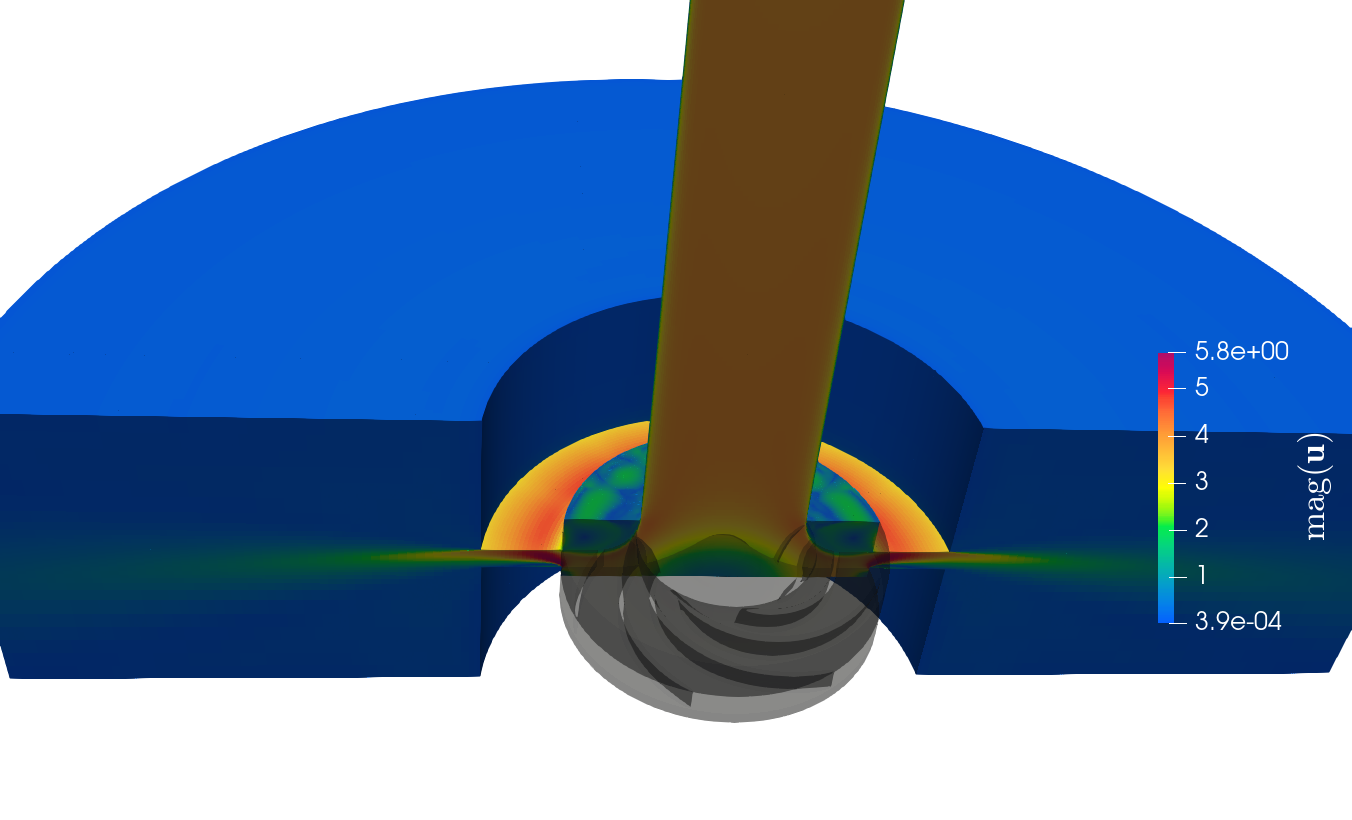
\includegraphics[width=0.9\linewidth]{figures/Pump_sim2.png}

        \begin{columns}
            \begin{column}{0.542\textwidth}
        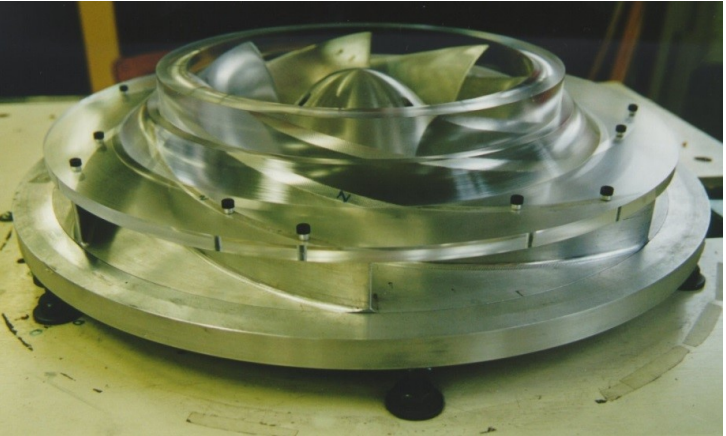
\includegraphics[width=\linewidth]{figures/RESEDA_benchmark.png}
            \end{column}
            \begin{column}{0.458\textwidth}
        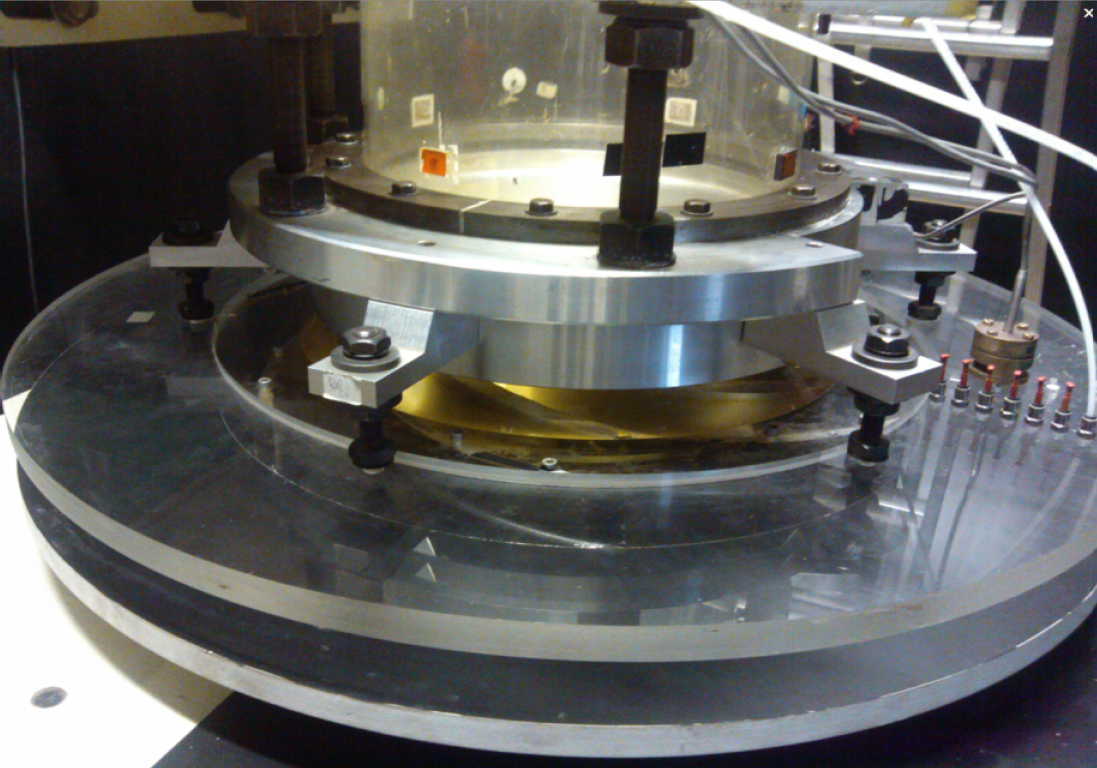
\includegraphics[width=\linewidth]{figures/image1.png}
            \end{column}
        \end{columns}
    \end{column}
\end{columns}

\end{frame}

\begin{frame}{Introduction \& context}

\begin{columns}
    \begin{column}{0.4\textwidth}
        \centering
        %\vspace{0.3cm}
        % 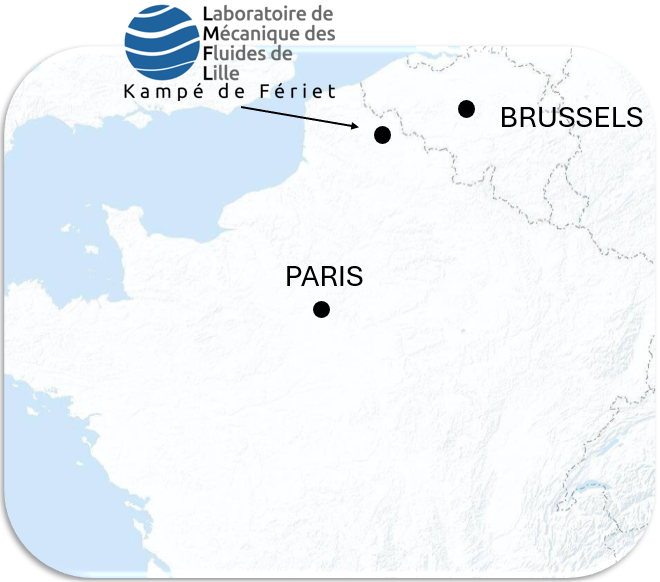
\includegraphics[scale=0.25]{figures/Map_LMFL.png}
        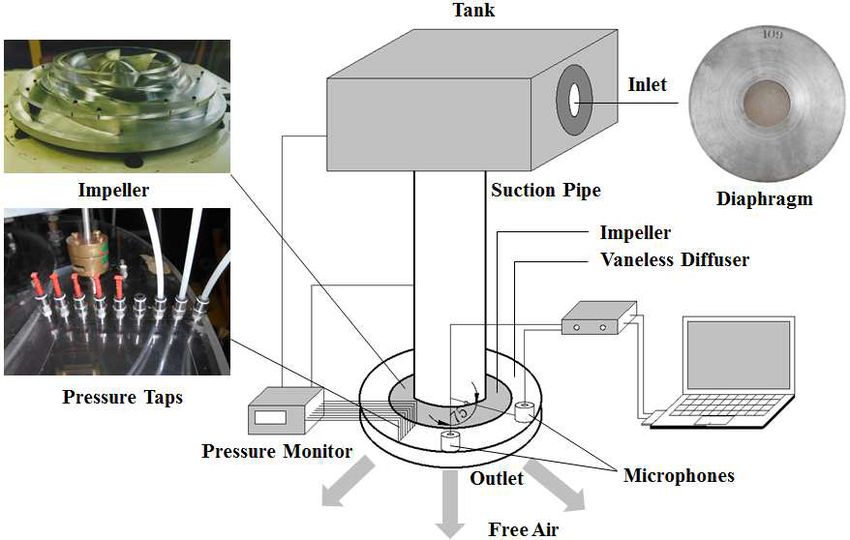
\includegraphics[scale=0.2]{figures/setting_centrifugalPump.png}
        \tiny{(extracted from Dazin et al.)}
    \end{column}

    \pause
    
    \begin{column}{0.6\textwidth}
        \begin{tabular}{cc}
            \structure{\textbf{SHF}} (\emph{Société Hydrotechnique de France}) \structure{\textbf{impeller}}

                \centering
                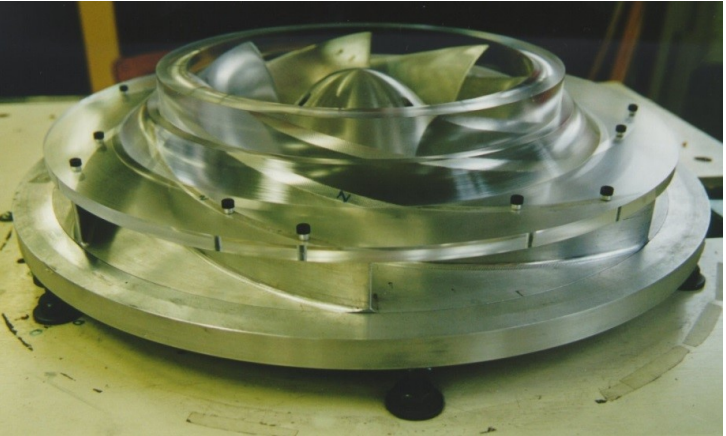
\includegraphics[width=0.5\textwidth]{figures/RESEDA_benchmark.png}
            \item Several kinds of \structure{\textbf{vaned and vaneless diffusers}} $\rightarrow$ in this work we model the pump with a \textcolor{red}{vaneless diffuser and aspect ratio $\Gamma=1.5$}
        
            \begin{tabular}{cc}
                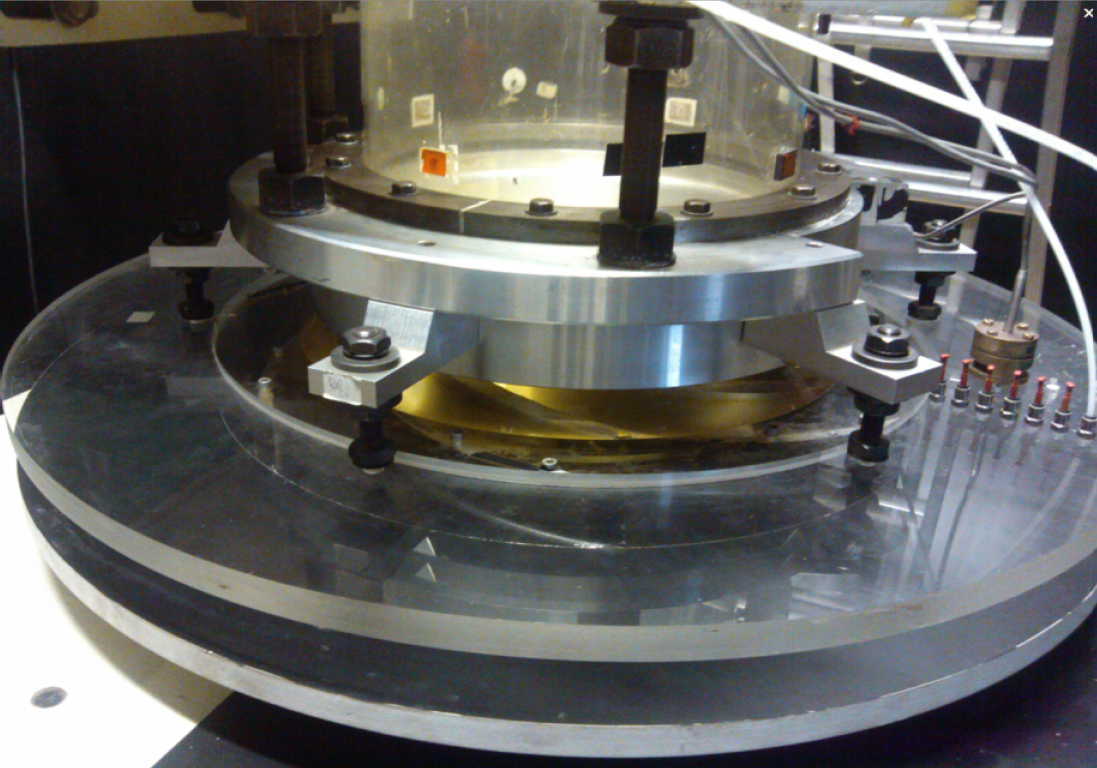
\includegraphics[scale=0.11]{figures/image1} & 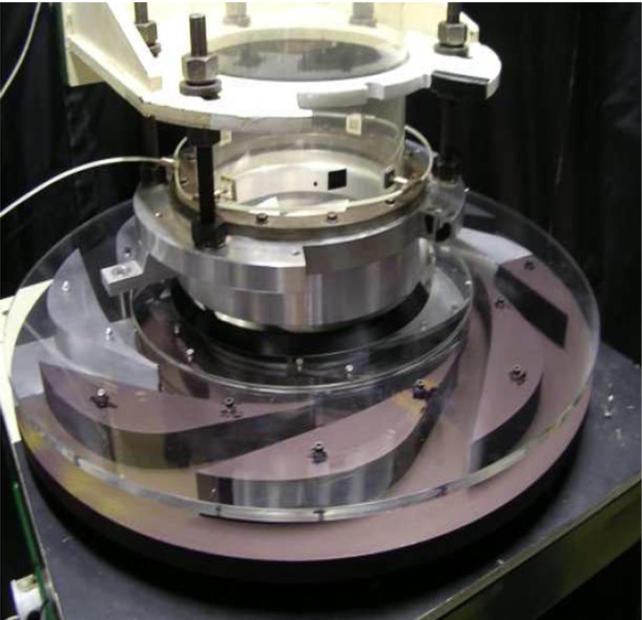
\includegraphics[scale=0.15]{figures/bancEssais.png}
            \end{tabular}
        
        \end{itemize}}

        \only<2-3>{\tiny{\begin{tabular}{c c c}
        \multicolumn{3}{c}{\textbf{SHF Impeller characteristics}} \\ \hline 
         $R_1$ & Tip inlet radius & $141.1\,mm$  \\
         $R_2$ & Outlet radius & $257.5\,mm$ \\ 
         $Z$ & Number of blades & $7$ \\
         $Q_d$ & Design flow rate & $0.236\,m^3/s$ \\
         $K$ & Mean blade thickness & $9\,mm$ \\
         $\Omega$ & Rotating velocity & $1\,200\,rpm$ \\ 
         $\beta_2$ & Outside blade angle (from peripheral velocity $U=R_2\Omega$) & $22.5^{\circ}$ \\ \hline \hline
        \multicolumn{3}{c}{\textbf{Vaneless diffuser characteristics}} \\ \hline
         $b_3$ & Diffuser width & $38.5\,mm$ \\
         $R_3$ & Inlet radius (without leakage, i.e., $R_3=R_2$) & $257.5\,mm$ \\
         $R_4$ & Diffuser outlet radius & $385.5\,mm$ \\
         $t$ & Thickness of the upper and lower sections of the diffuser & $20\,mm$
        \end{tabular}}

        \onslide<3->
        \vspace{0.5cm}
        \centering
        
\includegraphics[scale=0.5]{figures/QUESTION_CFD_pump.png}
        
        \centering
        \textcolor{red}{\textbf{\normalsize{OpenFOAM\_v9 !}}}}
        
    \end{column}
\end{columns}
    
\end{frame}

\section{Modeling via an Immersed Boundary Method (IBM)}

\begin{frame}{Modeling via an Immersed Boundary Method (IBM)}

\begin{center}
    \textbf{IMMERSED BOUNDARY METHOD (IBM)}
\end{center}

\begin{itemize}
    \item The impeller features a highly complex geometry, making it \structure{\textbf{challenging to mesh accurately}} using native OpenFOAM tools such as \texttt{snappyHexMesh} or \texttt{cfMesh}

    \item \structure{\textbf{Commercial meshing software}} may become necessary \\

    \begin{center}
    \begin{columns}
        \begin{tabular}{ccc}
            
\includegraphics[scale=0.1]{figures/logos_softwareMesh/AG_logo.jpg} &
            
\includegraphics[scale=0.1]{figures/logos_softwareMesh/Ansys.png} &
            
\includegraphics[scale=0.1]{figures/logos_softwareMesh/PointwiseWTAG_WL_SCREEN.jpg}
        \end{tabular}
    \end{columns}
    \end{center}

    \item For unsteady simulations, \structure{\textbf{remeshing}} at each time step to account for the motion of the impeller \structure{\textbf{can be costly}}

\end{itemize}

\pause 
\vspace{1cm}

    \begin{columns}
        \begin{column}{0.5\linewidth}
            \centering
            $Re_\Omega=\cfrac{R_2^2 \Omega}{\nu} = 5.53\times10^5$ \textrm{\textbf{(turbulent)}}
        \end{column}
        \begin{column}{0.5\linewidth}
            \centering
            $Ma = \cfrac{R_2 \Omega}{c} = 0.095$ \textrm{\textbf{(incompressible)}}
        \end{column}
    \end{columns}

\centering
\textbf{Steady-state} conditions $\rightarrow$ \texttt{simpleFoam\_penalization}
\end{frame}

\begin{frame}{Modeling via an Immersed Boundary Method (IBM)}

\begin{block}{\structure{\textbf{Penalization IBM:}}}
    continuous penalty IBM for incompressible flows $\Rightarrow$ definition of a local \structure{direct forcing term} $\boldsymbol{f}_P$ within the Navier--Stokes equations to \textbf{enforce the boundary conditions at the immersed wall} $\boldsymbol{(ib)}$
\end{block}

\vspace{-0.2cm}
\begin{equation*}
\boldsymbol{\nabla} \cdot (\boldsymbol{u}\boldsymbol{u}) = -\nabla p + \nu \nabla^2 \boldsymbol{u}  \overbrace{-\frac{\xi}{\eta} \left(\boldsymbol{u} - \boldsymbol{u_{ib}} \right)}^{\boldsymbol{f}_P}
\end{equation*}


\begin{columns}
    \begin{column}{0.5\textwidth}
        \centering
        \only<1>{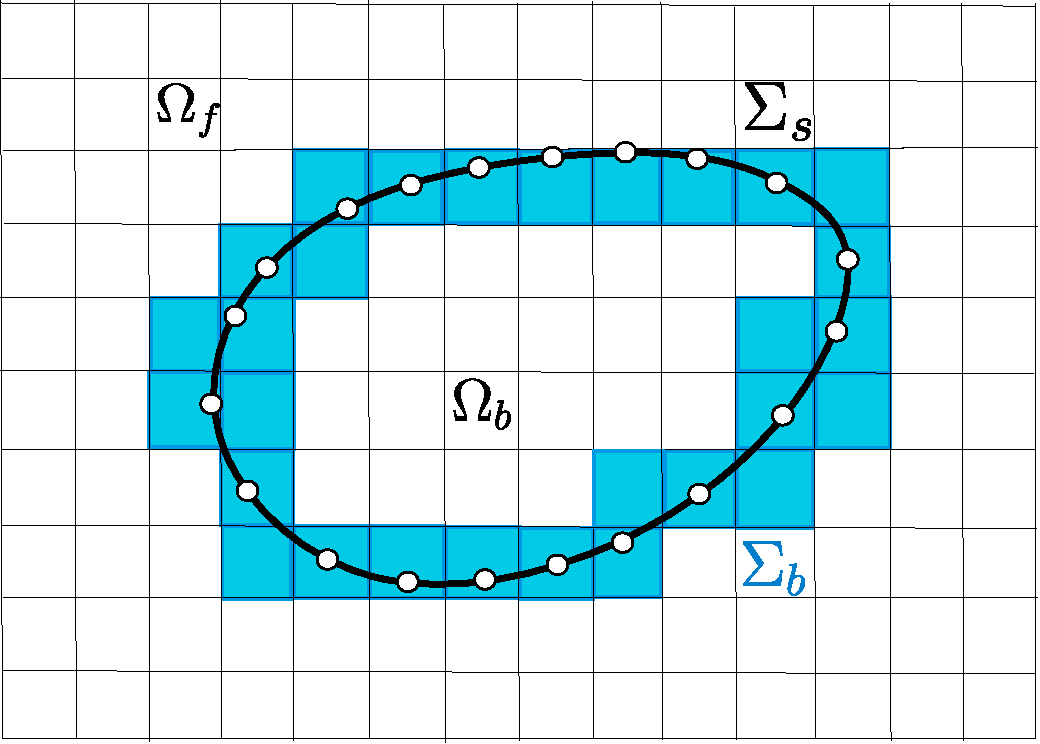
\includegraphics[scale=0.25]{figures/IBM_Mesh.pdf}}
        \only<2>{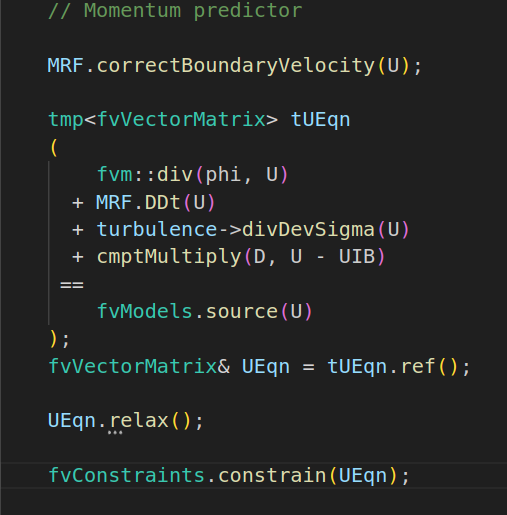
\includegraphics[scale=0.25]{figures/implicit_forcing.png}}
    \end{column}
    \begin{column}{0.5\textwidth}
        \begin{equation*}
         \xi = \left\{
        \begin{array}{ll}
        0 & \textrm{if } \boldsymbol{x} \in \Omega_f \\
        1 & \textrm{if } \boldsymbol{x} \in (\Sigma_b \cup \Omega_b)
        \end{array} \right.
        \end{equation*}

        \colorbox{blue!20}
        {\parbox{0.85\textwidth}
        { \centering when $\eta \rightarrow 0$, \\ \textbf{IBM field = body-fitted field}}}

        \vspace{0.2cm}
        
        \footnotesize{... but too low values of $\eta$ may lead to flow instabilities...}
        
    \end{column}
\end{columns}
    
\end{frame}

\begin{frame}{Modeling via an Immersed Boundary Method (IBM)}

\begin{columns}
    \begin{column}{0.6\linewidth}
        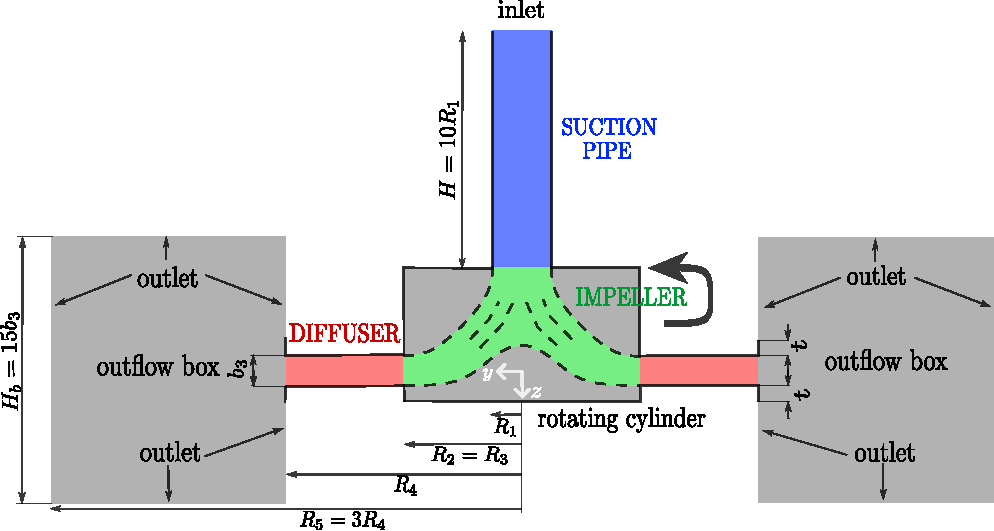
\includegraphics[scale=0.5]{figures/RESEDA_sketch.pdf}

        \footnotesize{\begin{itemize}
            \item \textbf{Boundary conditions:}
                \begin{itemize}
                    \item Inlet $\rightarrow$ \texttt{flowRateInletVelocity}
                    \item Outlet $\rightarrow$ \texttt{fixedValue} (for the pressure $p$)
                \end{itemize}
            \item \textbf{IBM:} need for an additional surrounding \structure{computational domain around the impeller}
        \end{itemize}}
    \end{column}

    \pause 
    
    \begin{column}{0.4\linewidth}

    \footnotesize{
        \begin{itemize}
            \item CAD with the impeller geometry:
        \end{itemize}
        \centering
        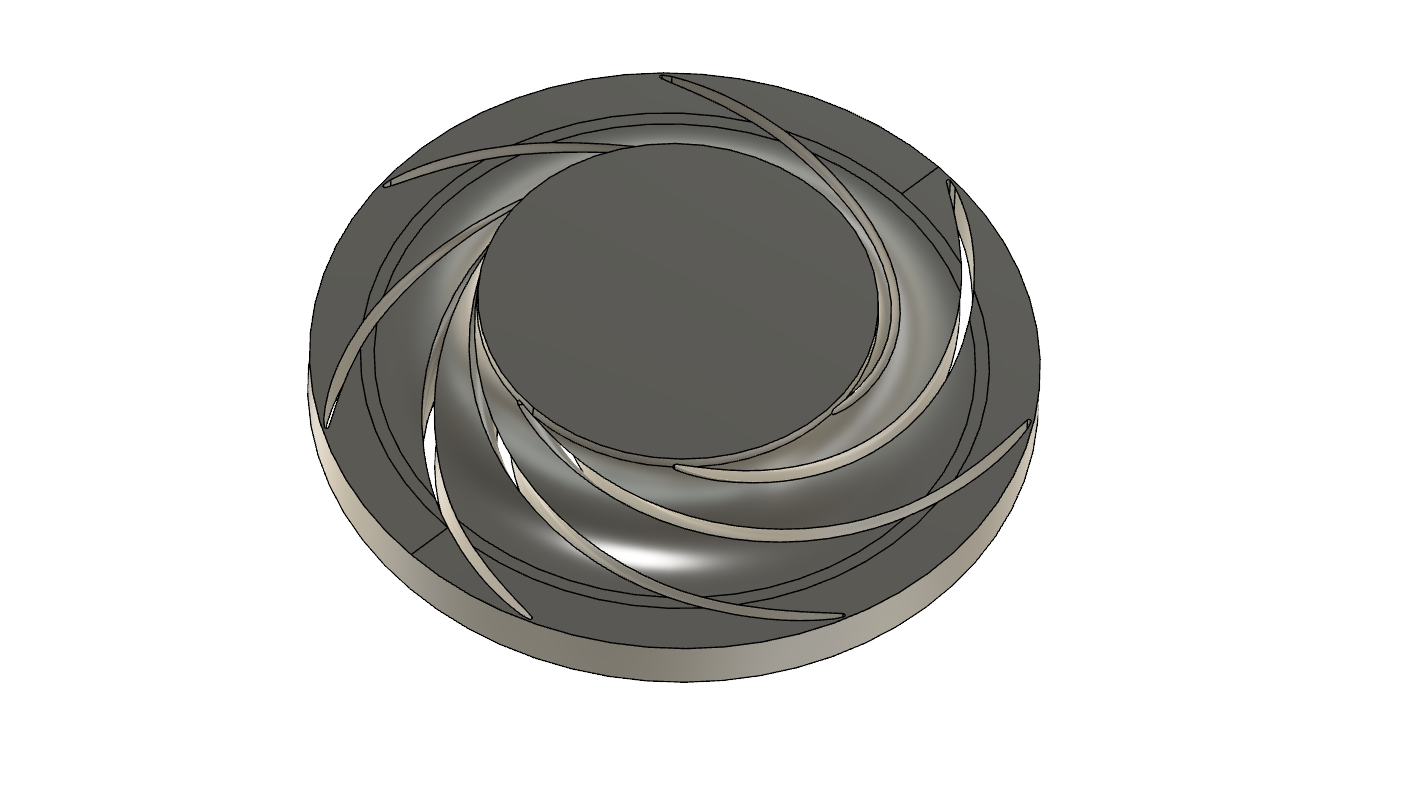
\includegraphics[scale=0.075]{figures/CAD_Impeller v2.png}

        \begin{itemize}
            \item Building of the surrounding cylinder:
        \end{itemize}

        \begin{itemize}
            \item Boolean operation to identify the solid regions (cellRegion via \texttt{topoSetDict} from \texttt{.stl} file):
        \end{itemize}
        \begin{center}
        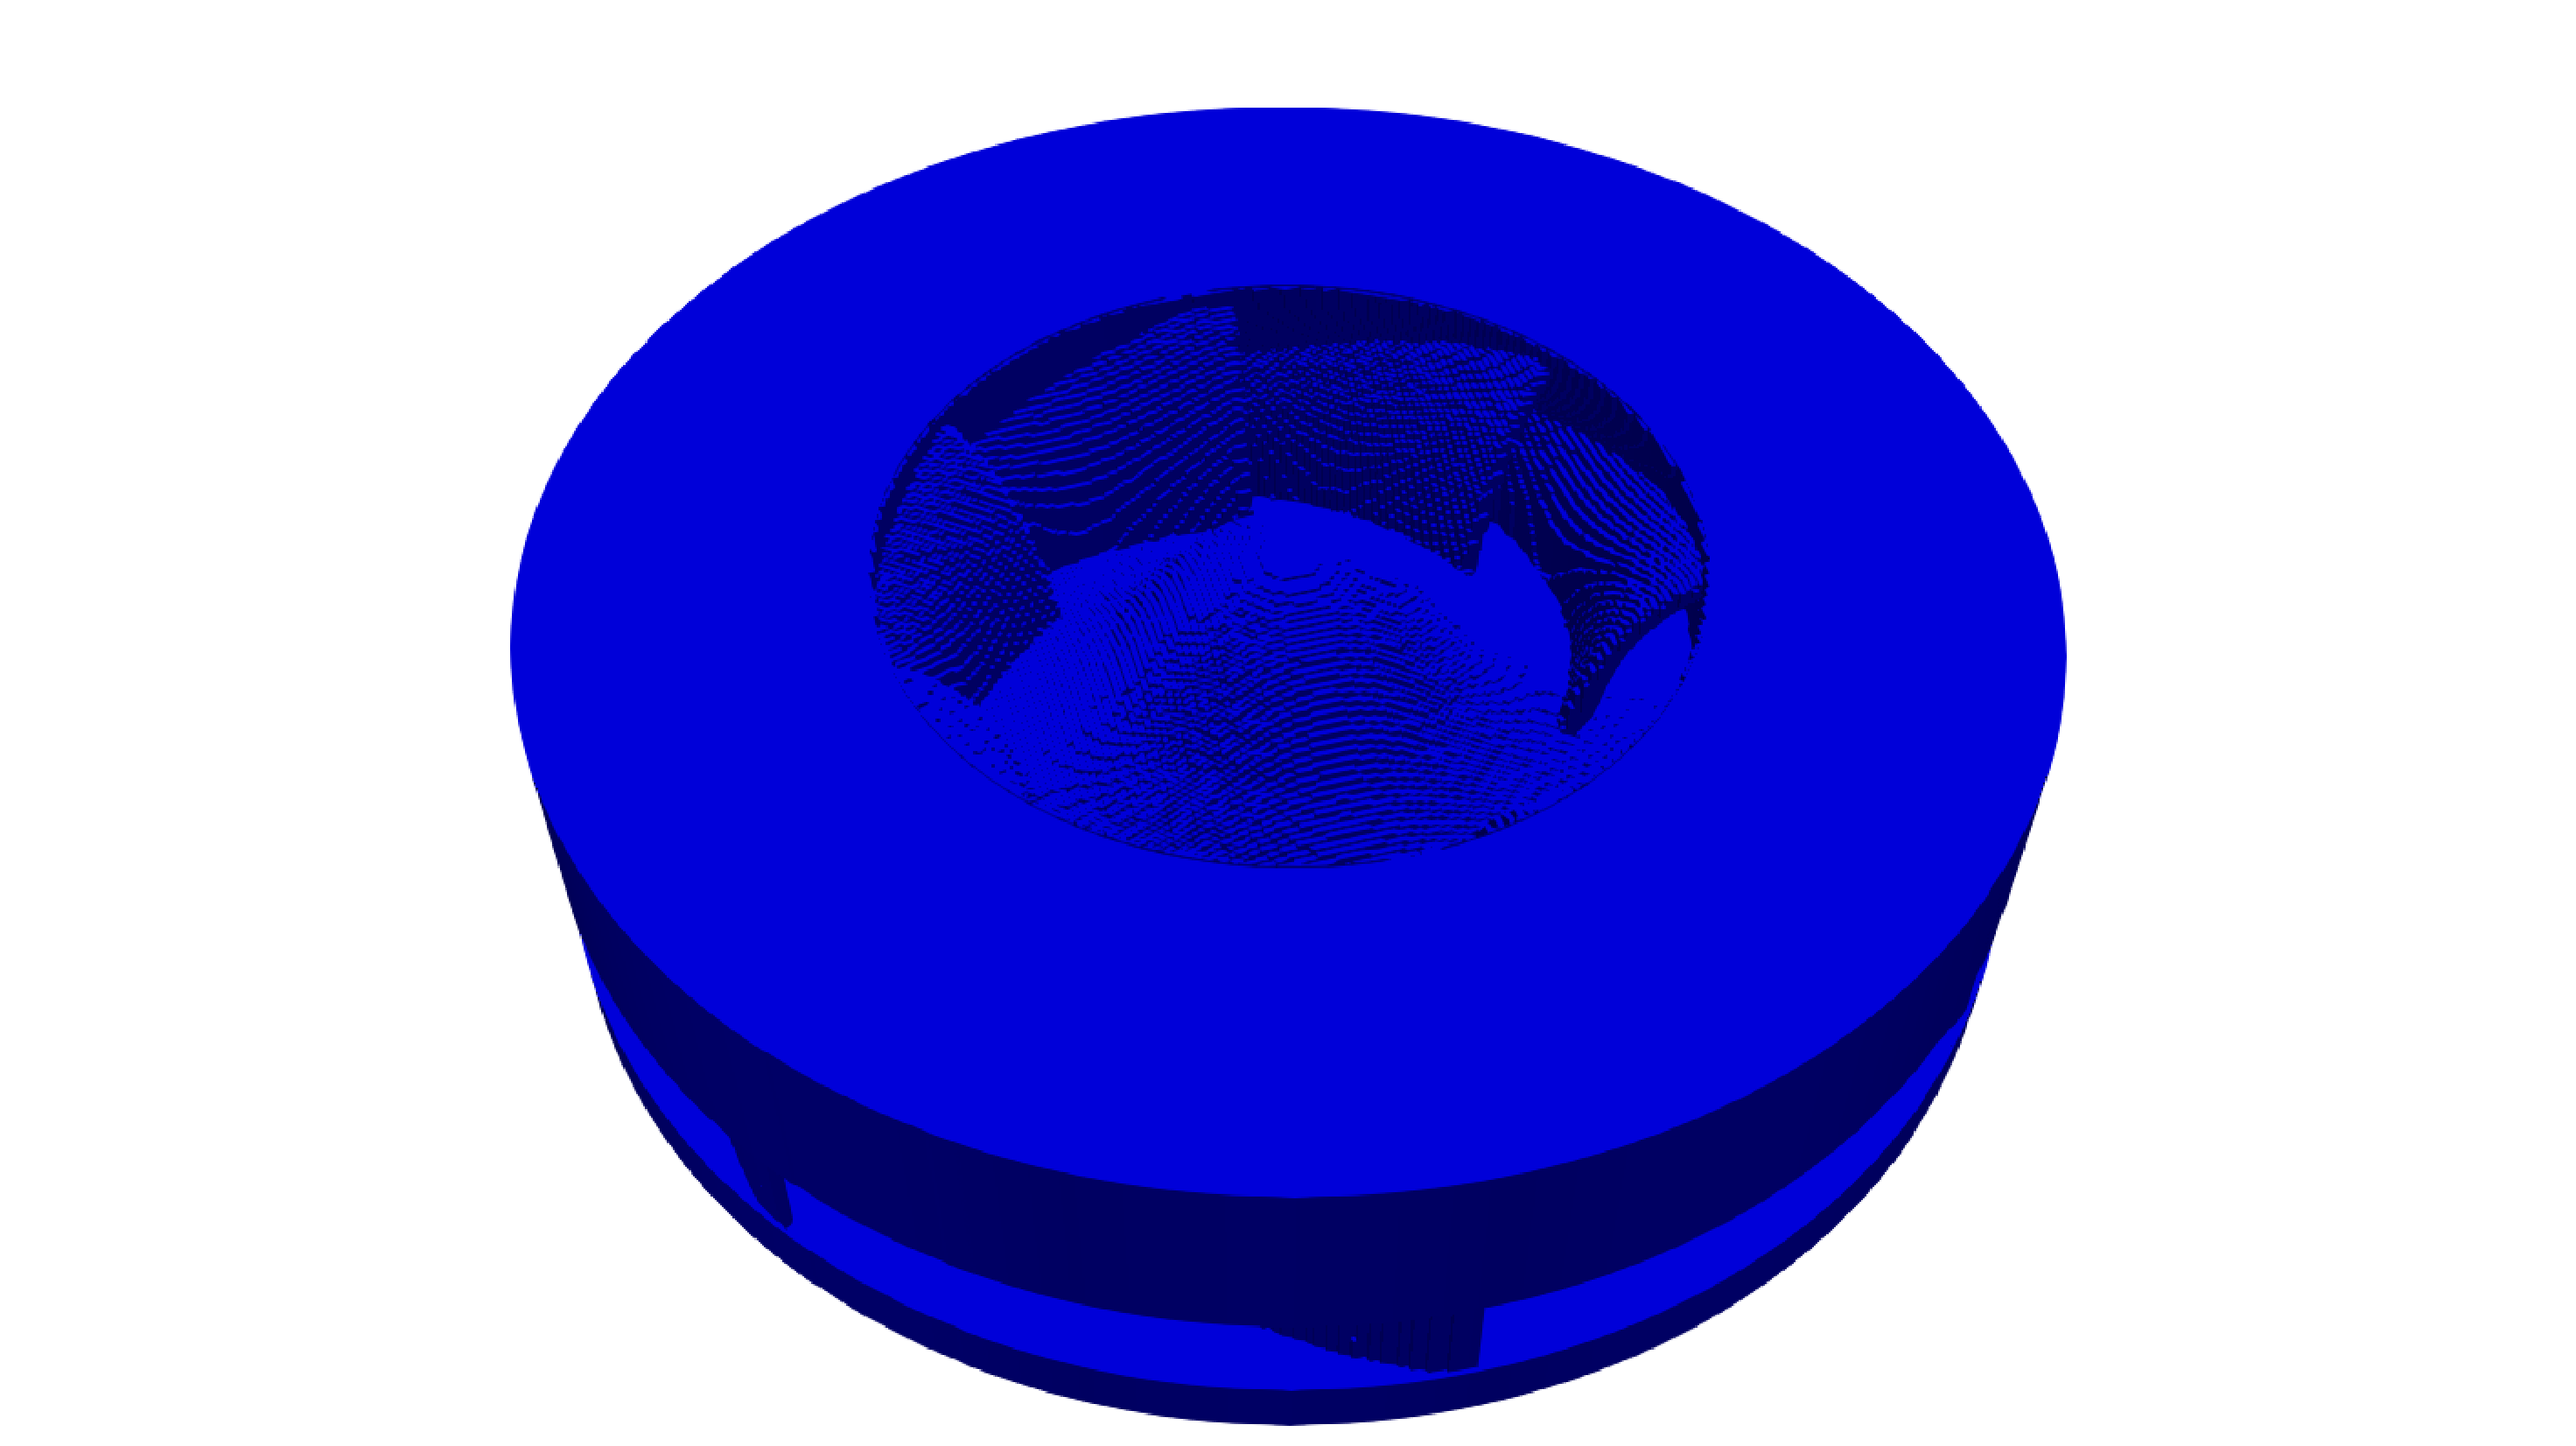
\includegraphics[scale=0.075, trim={0, 0, 0, 0}, clip]{figures/impeller_cells.pdf}
        \end{center}
    }
        
    \end{column}
\end{columns}
    
\end{frame}

\begin{frame}{Modeling via an Immersed Boundary Method}

\begin{itemize}
    \item The mesh is entirely defined through the \texttt{blockMeshDict} file
    \item All regions of the pump are constituted by \structure{\textbf{conformal blocks}}, with the only exception being the cutting faces between the suction pipe and the impeller, which are assumed by the \texttt{mergePatchPairs} function
\end{itemize}

\begin{columns}
        \begin{column}{0.5\linewidth}
     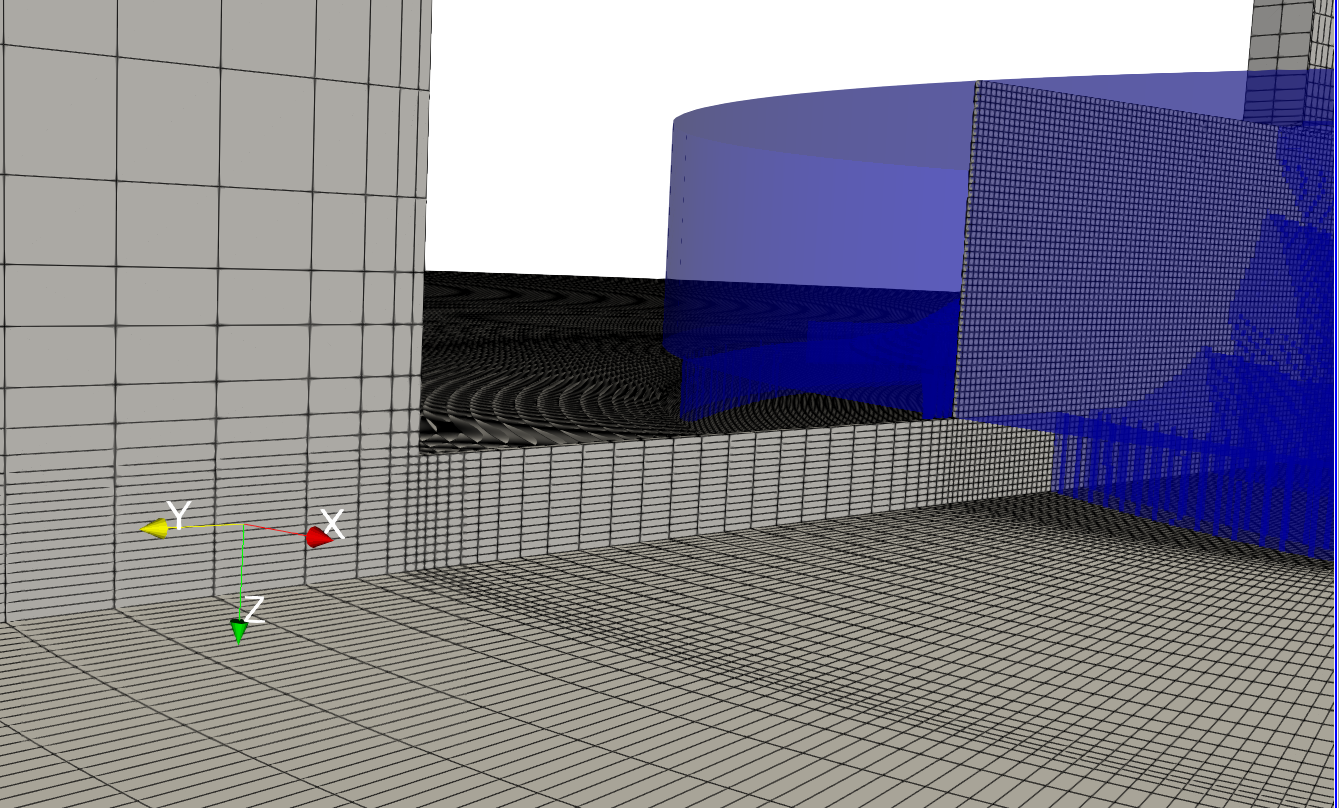
\includegraphics[width=\textwidth]{figures/mesh/blockMesh.png}
        \end{column}
        \begin{column}{0.5\linewidth}
    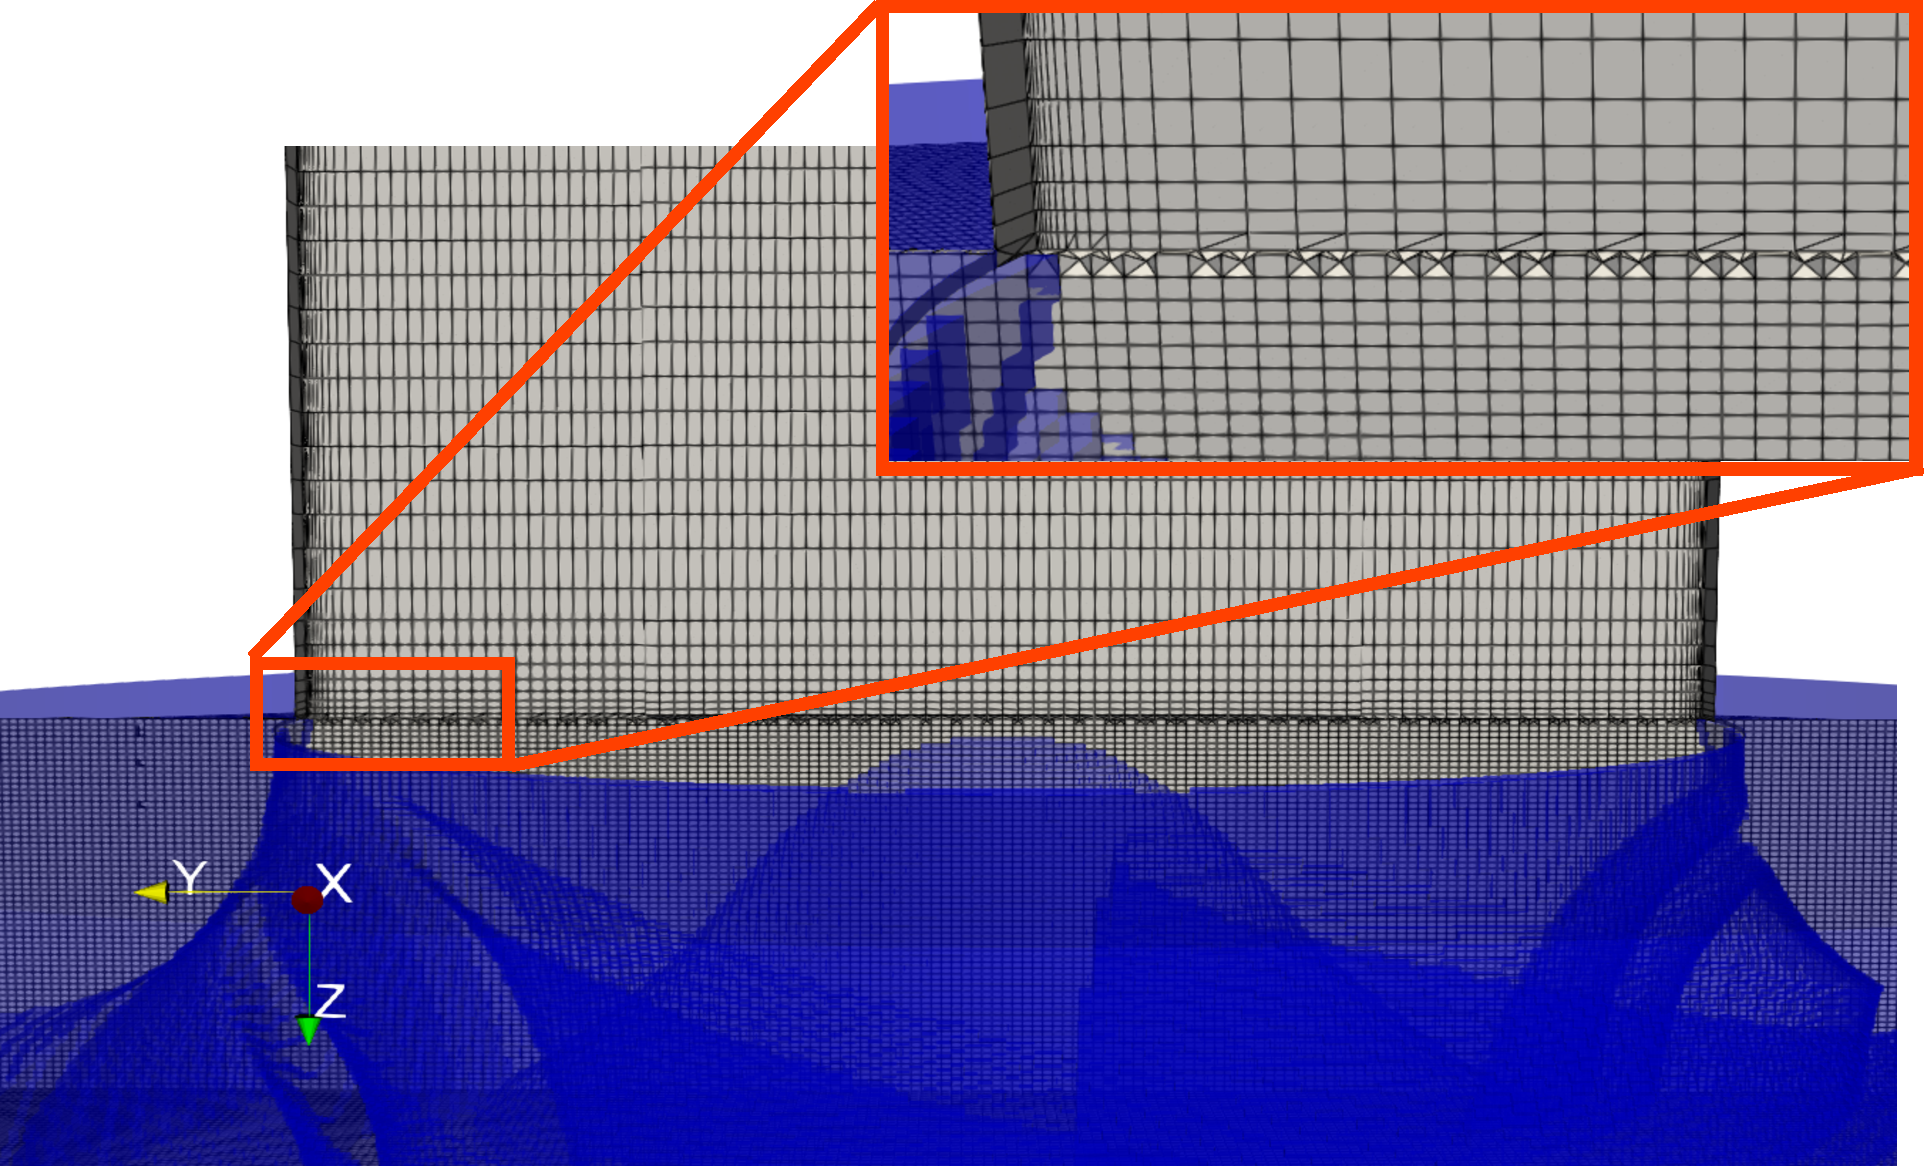
\includegraphics[width=\textwidth]{figures/mesh/frontalView.pdf}
        \end{column}
\end{columns}
    
\end{frame}

\begin{frame}{Modeling via an Immersed Boundary Method}

\begin{columns}
    \begin{column}{0.5\linewidth}
    \begin{itemize}[<+->]
        \item Steady-state simulation with the \structure{\textbf{Multiple Reference Frame (MRF)}} approach
        \item $\mathcal{K}-\omega$ SST model $\rightarrow$ Five penalty coefficients $\eta = (\boldsymbol{\eta_u}, \eta_\mathcal{K}, \eta_\omega)$

    \begin{eqnarray*}
        \boldsymbol{f}_{P_u} &= \frac{\xi}{\boldsymbol{\eta_u}} (\boldsymbol{u}-\boldsymbol{u_{ib}}) \rightarrow \boldsymbol{u_{ib}} &= \cancel{\boldsymbol{u}_r} + \boldsymbol{\Omega} \times \boldsymbol{r} \\
        \boldsymbol{f}_{P_\mathcal{K}} &= \frac{\xi}{\eta_\mathcal{K}} (\mathcal{K}-\mathcal{K}_{ib}) \rightarrow \mathcal{K}_{ib} &= 0 \\
        \boldsymbol{f}_{P_\omega} &= \frac{\xi}{\eta_\omega} (\omega-\omega_{ib}) \rightarrow \omega_{ib} &= (\omega_{vis}^2+\omega_{log}^2)^{1/2}
    \end{eqnarray*}
    where $\omega_{vis}=\frac{6 \nu}{\beta_1 y_{\mathrm{ref}}^2}$ and $\omega_{log} = \frac{\sqrt{\mathcal{K}}}{C_\mu \kappa y_\mathrm{ref}}$

    \vspace{0.5cm}

    \centering
    \texttt{kOmegaSST\_penalization}

        \end{itemize}

    \end{column}
    \begin{column}{0.5\linewidth}
        \centering
        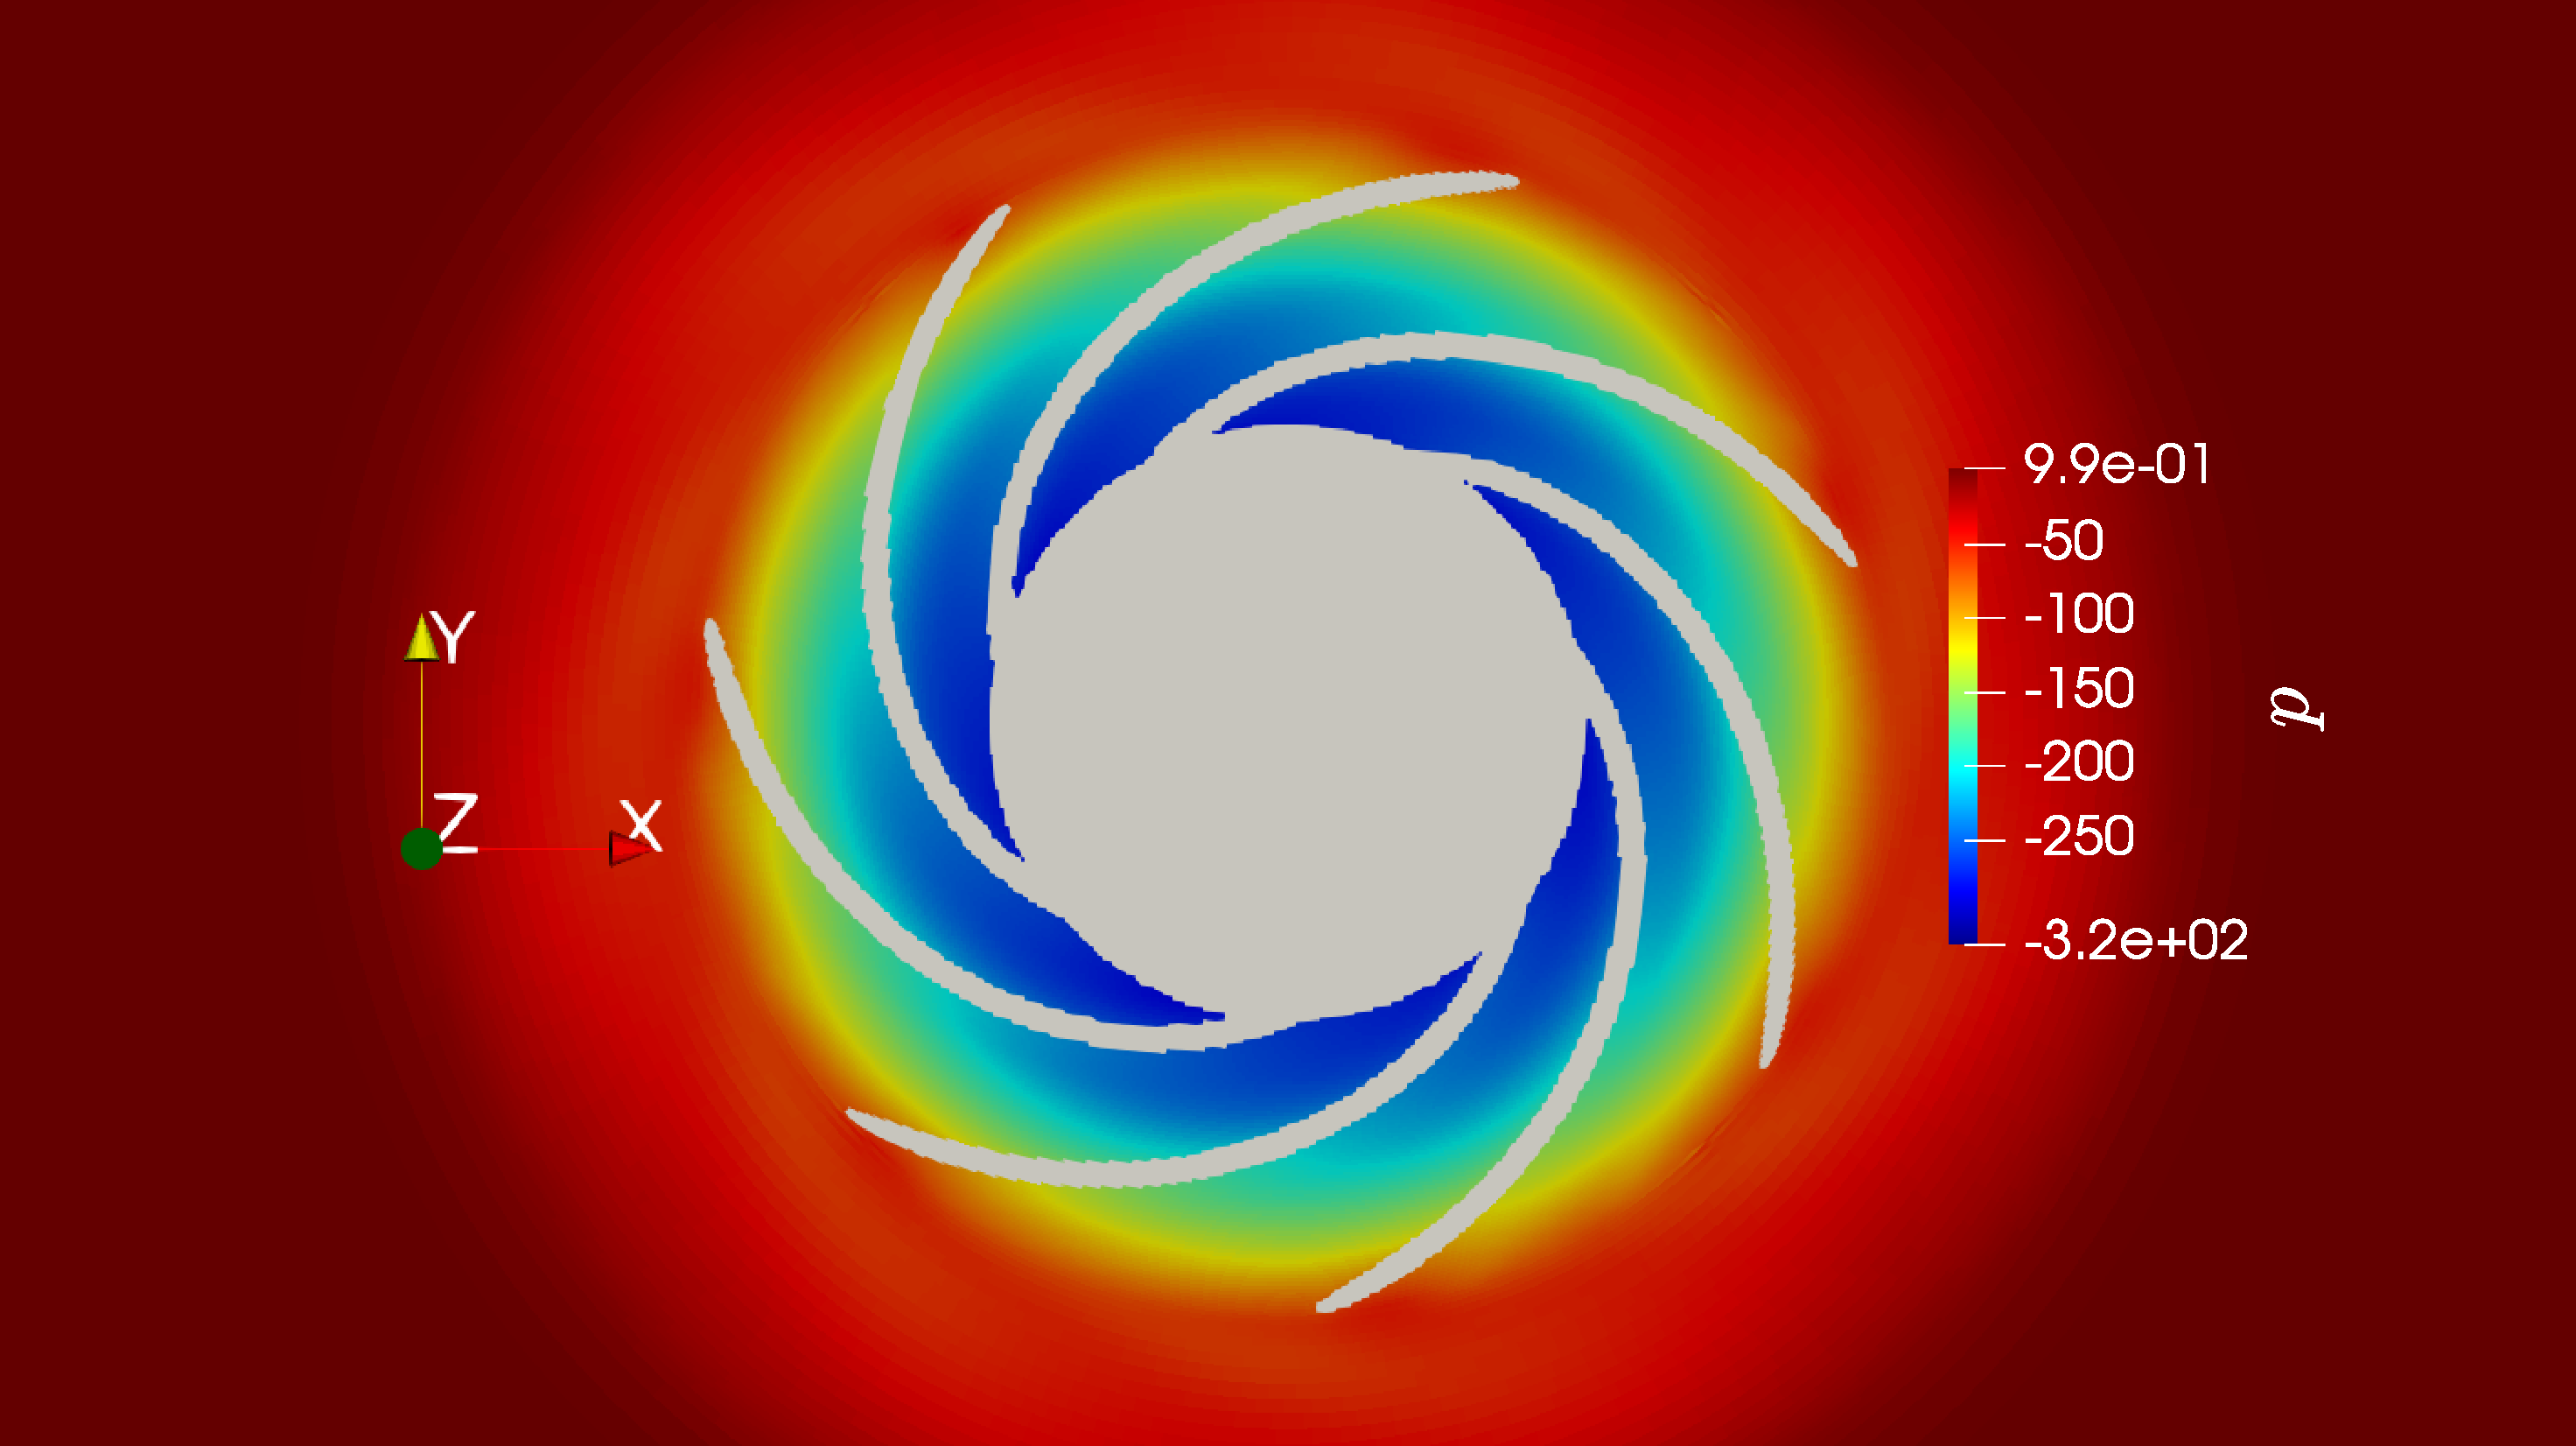
\includegraphics[width=0.8\textwidth]{figures/pressure_profile.pdf}
        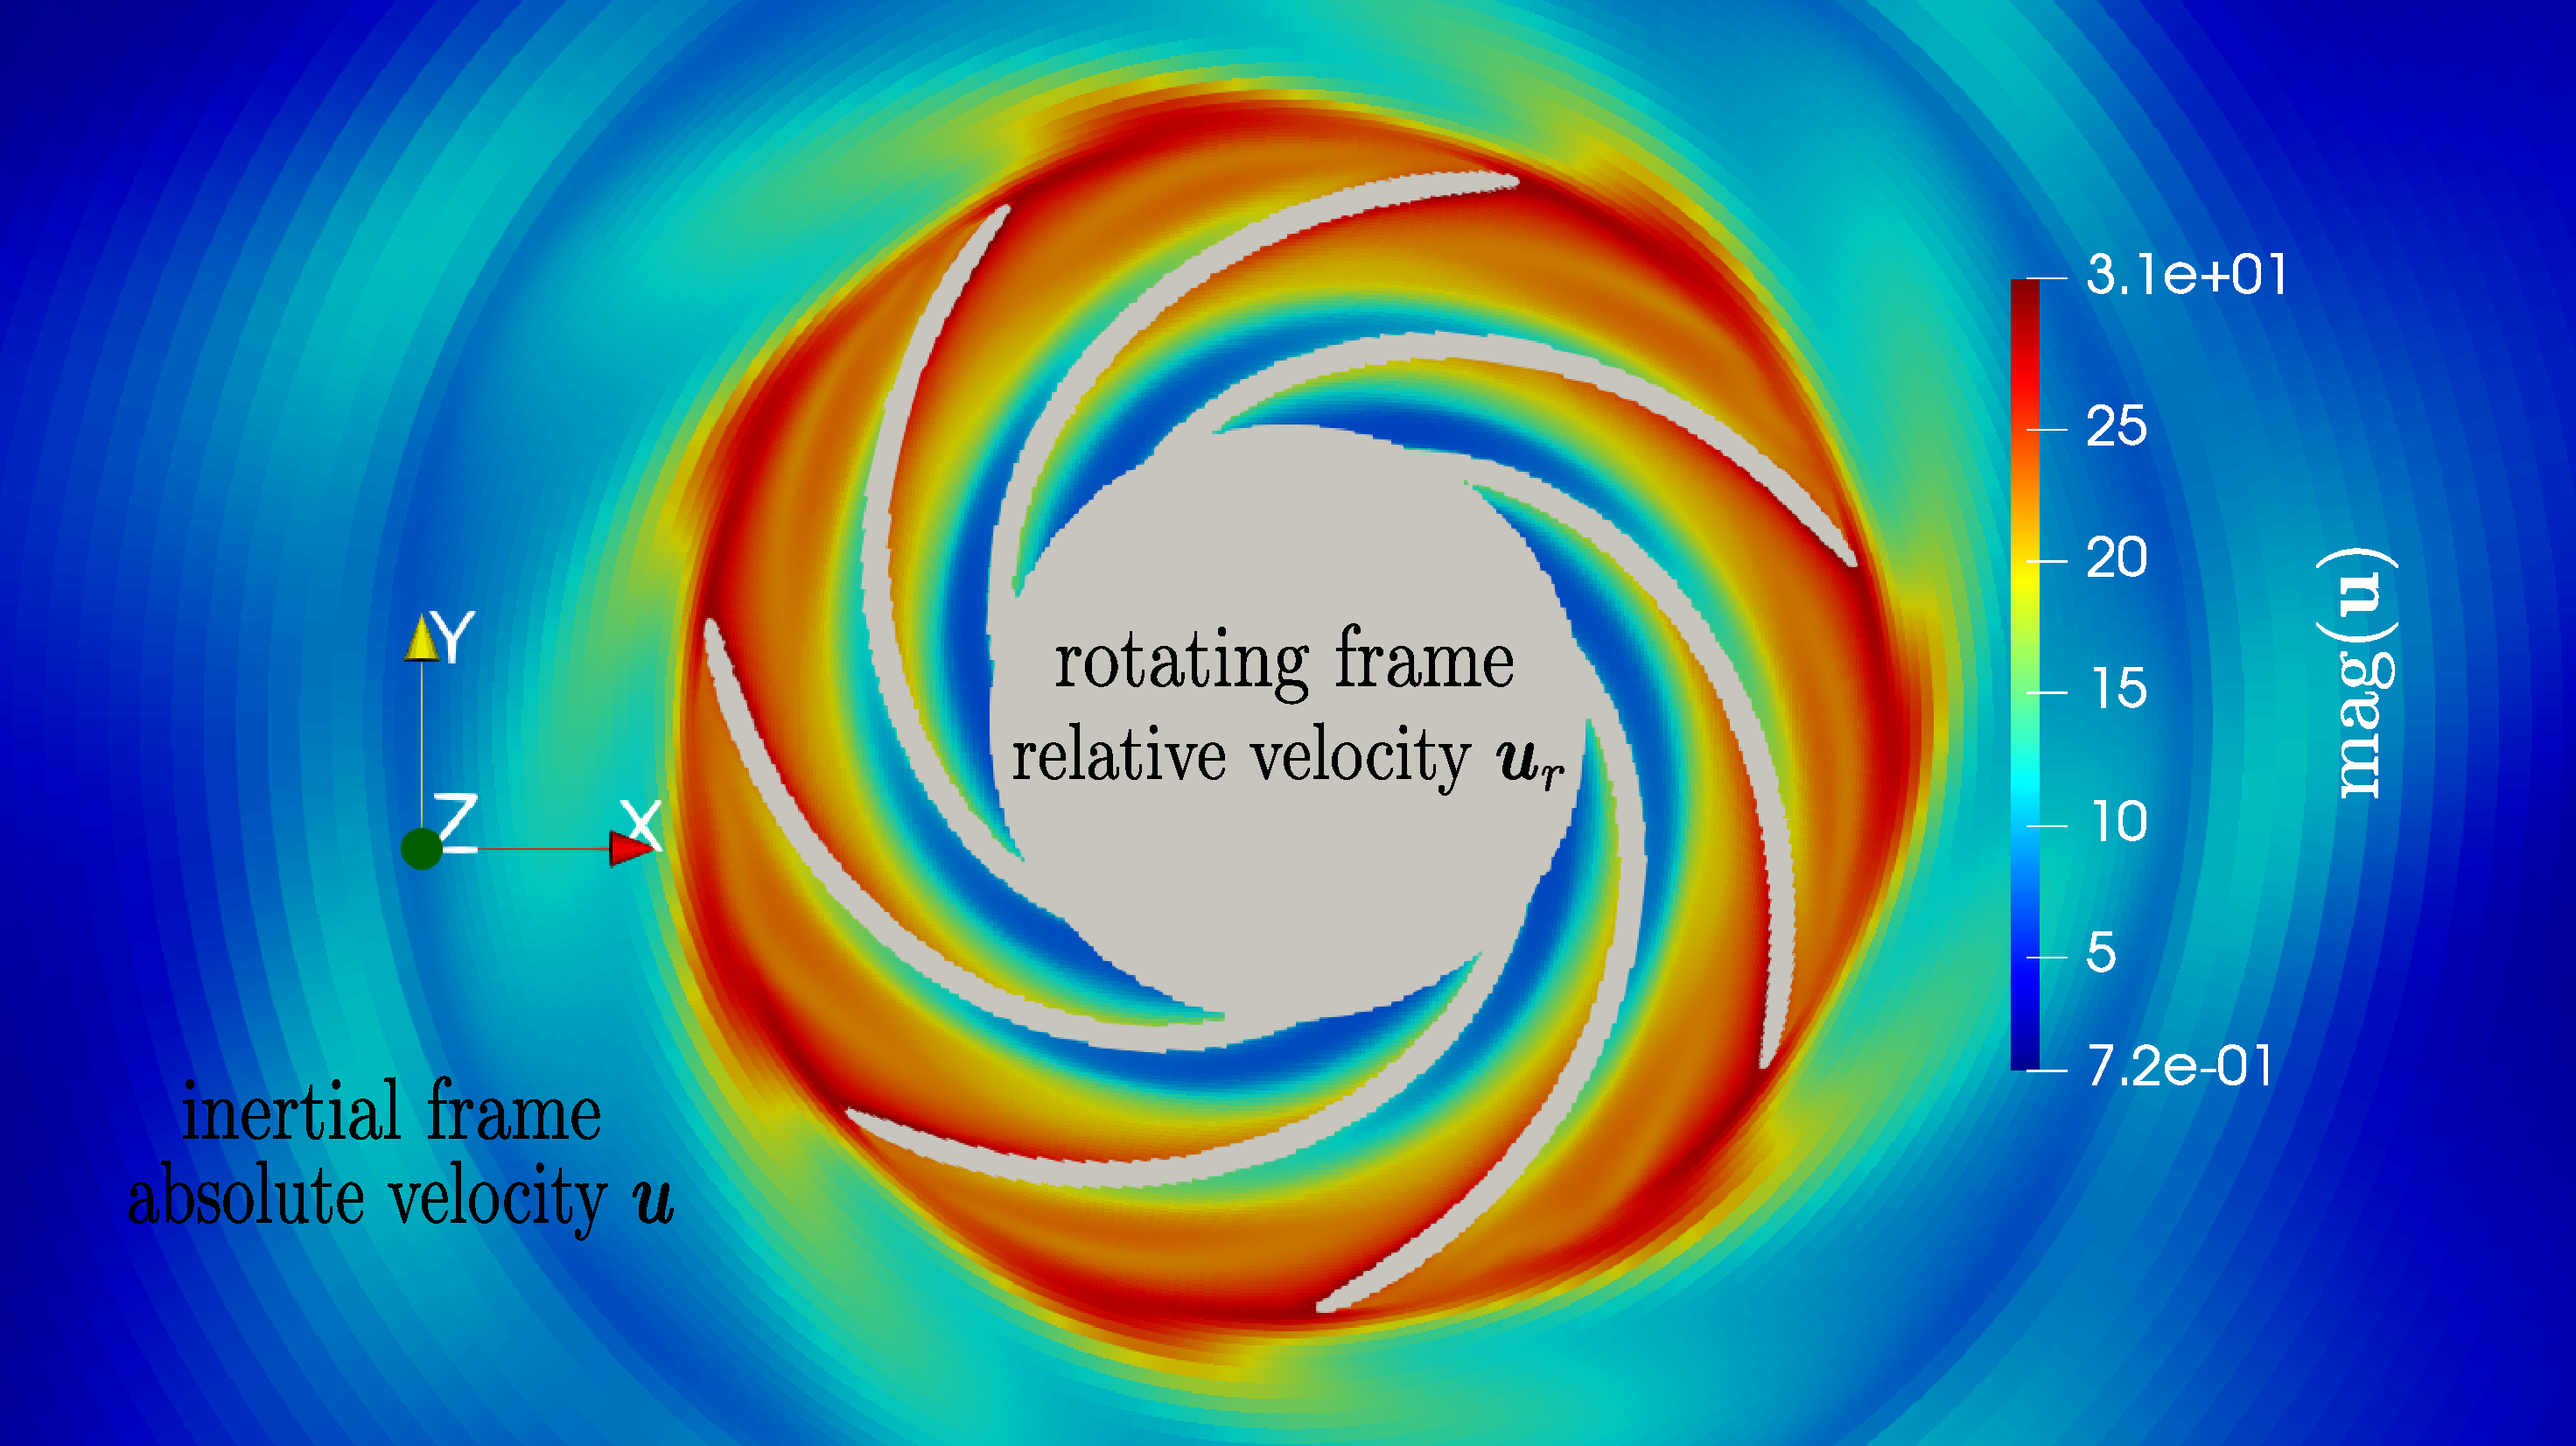
\includegraphics[width=0.8\textwidth]{figures/velocity_profile.pdf}
    \end{column}
\end{columns}
\end{frame}

\section{Preliminary results}

\begin{frame}{Preliminary results}

    \begin{columns}
        \begin{column}{0.5\linewidth}
            \begin{itemize}
                \item \structure{\textbf{Performance of the diffuser}} in agreement with pressure taps

                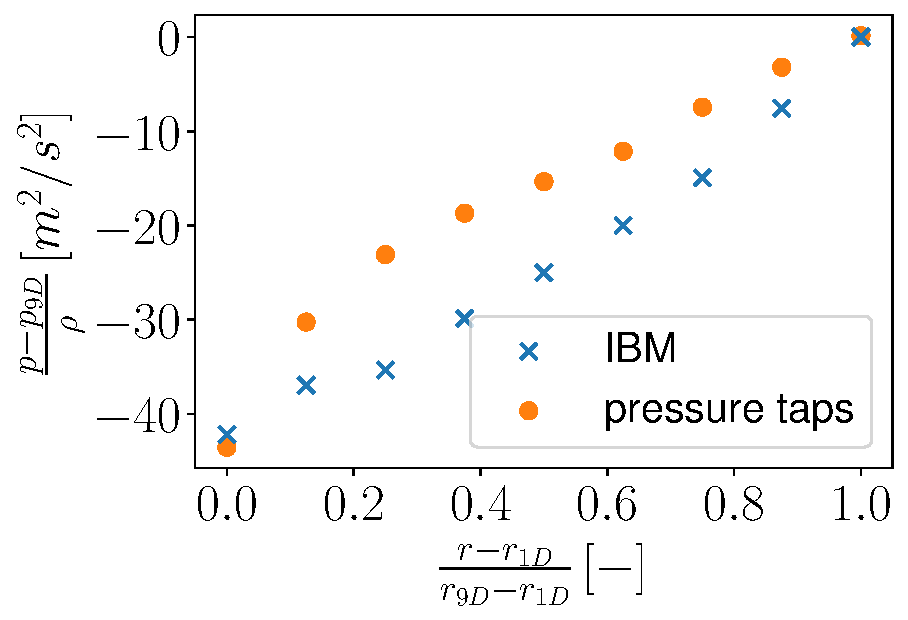
\includegraphics[scale=0.4]{figures/diffuser_performance.pdf}

                \item \structure{\textbf{Performance of the impeller}} still needs to be checked with different IBM coefficients $\eta$
            \end{itemize}
        \end{column}

        \pause 
        
        \begin{column}{0.5\linewidth}
            \centering
            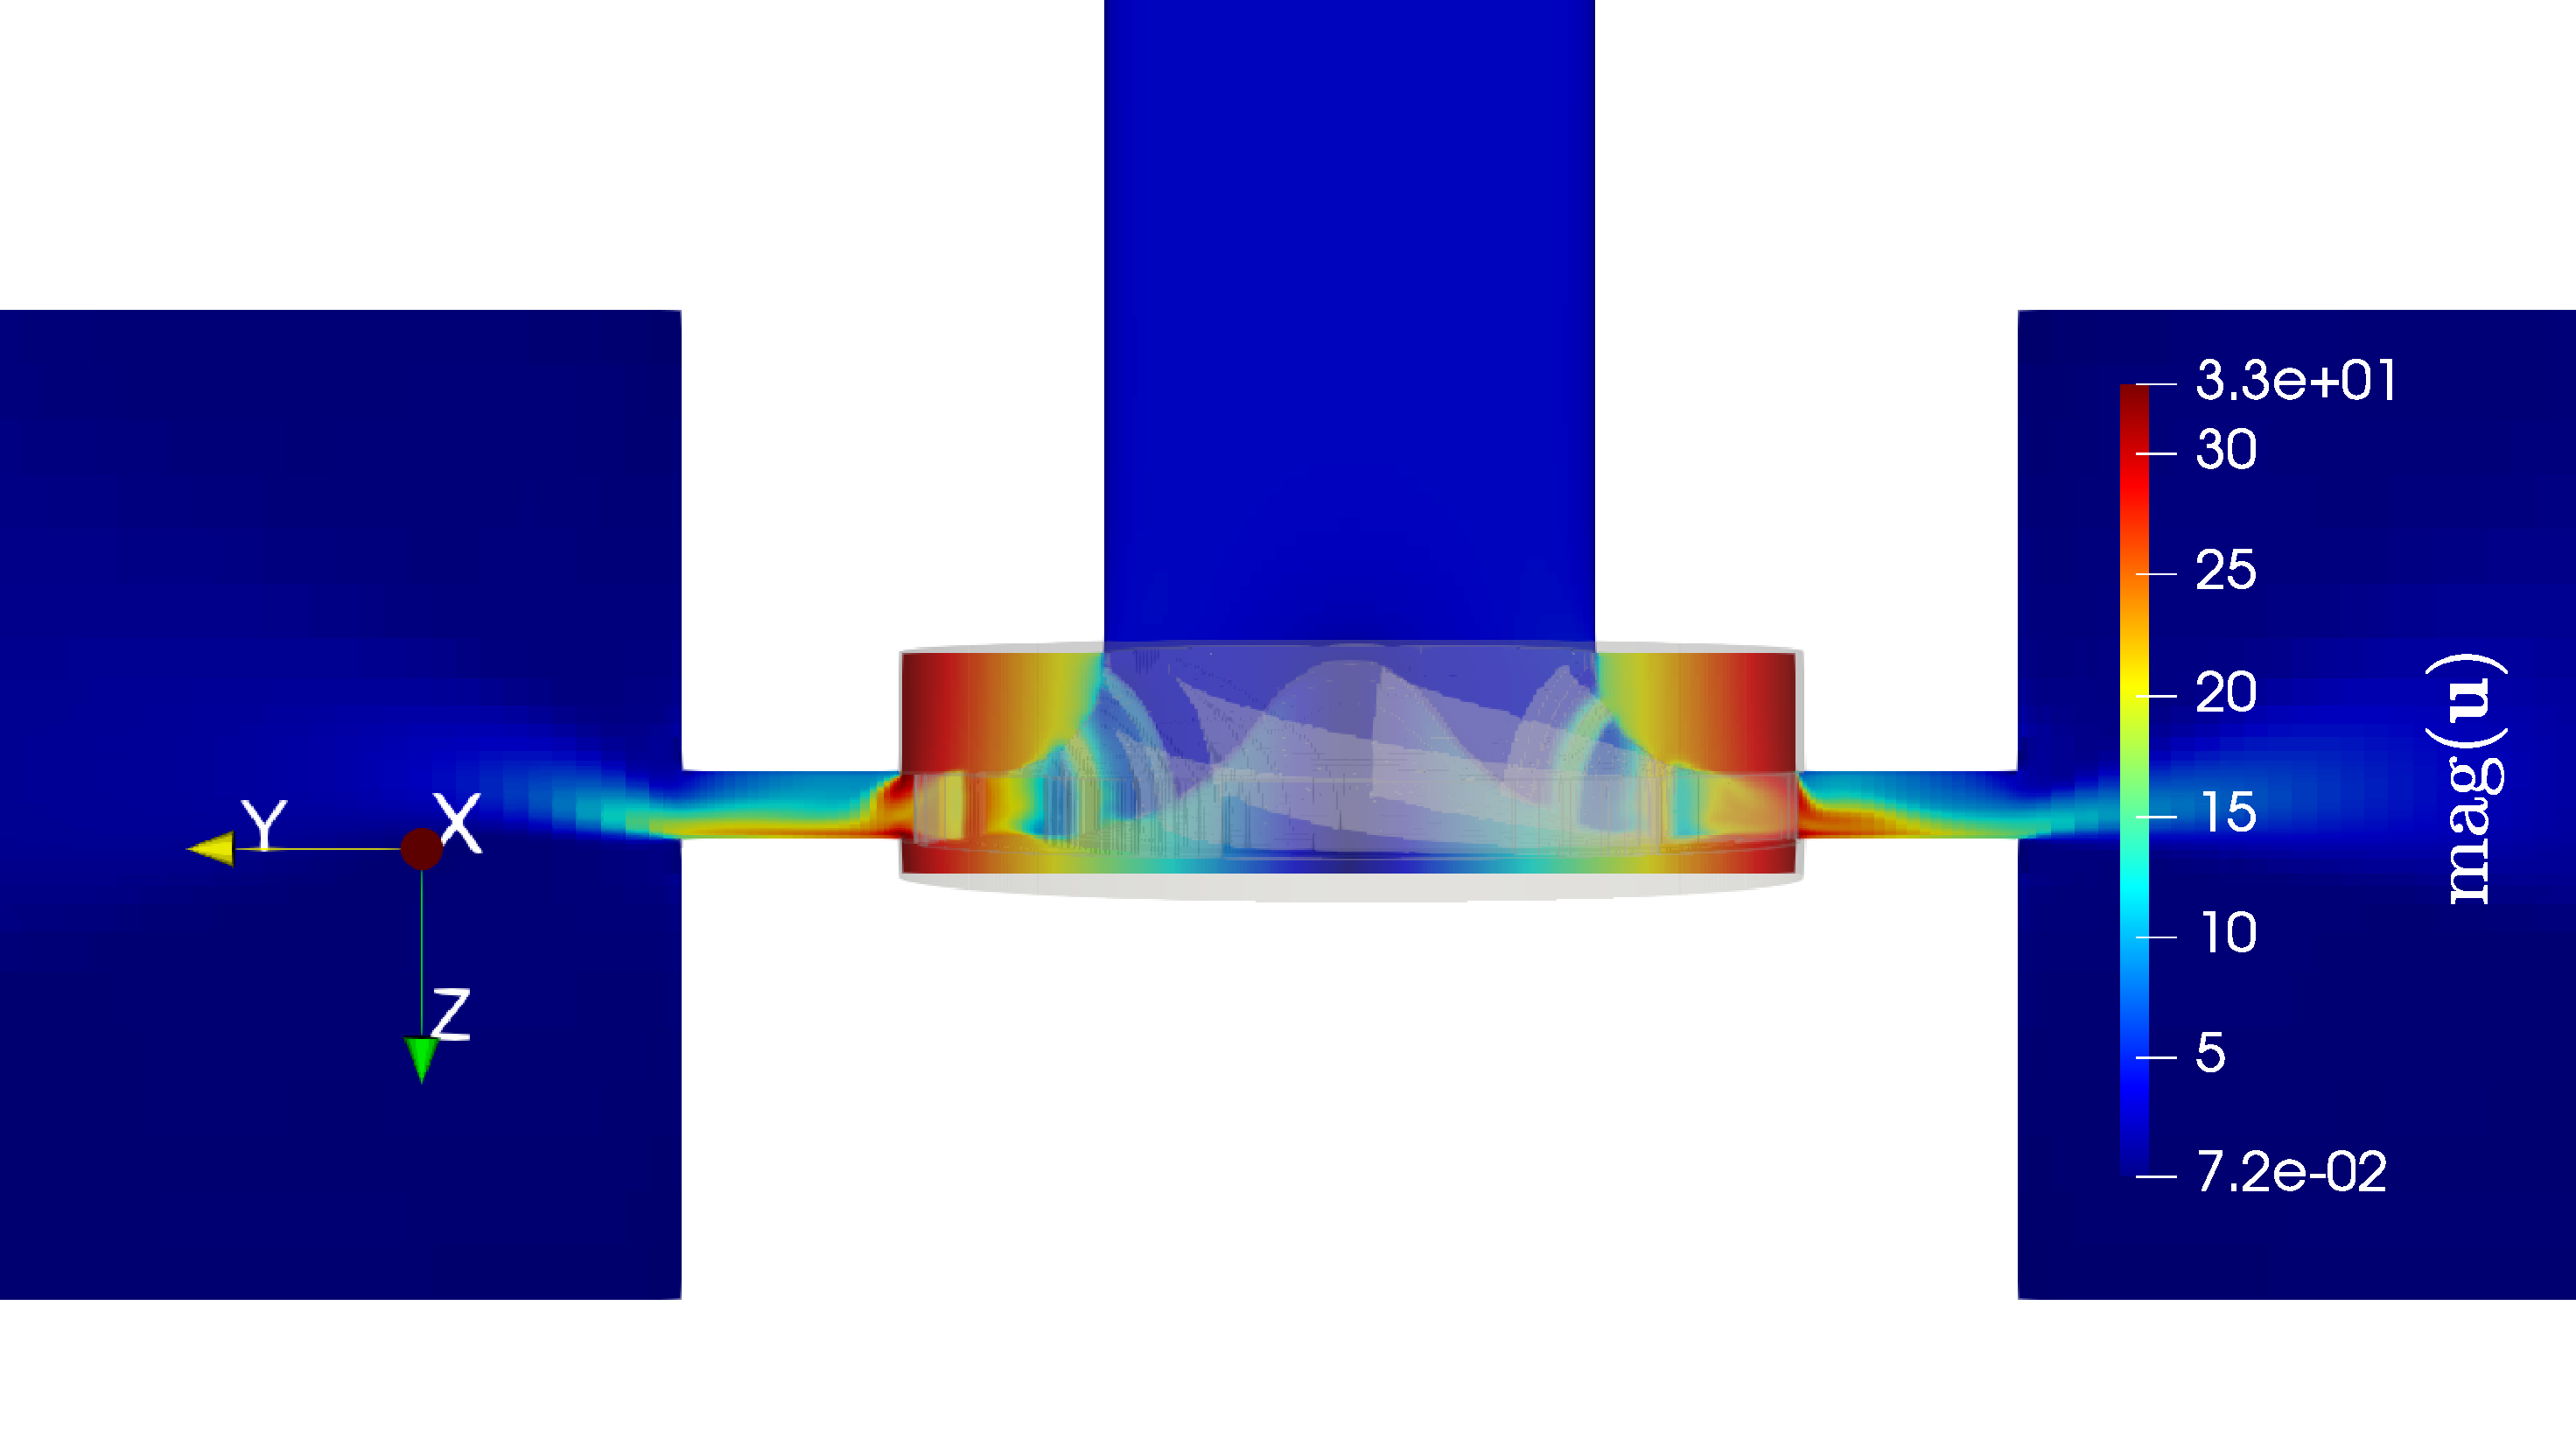
\includegraphics[width=0.9\textwidth]{figures/velocity_verProfile.pdf}
            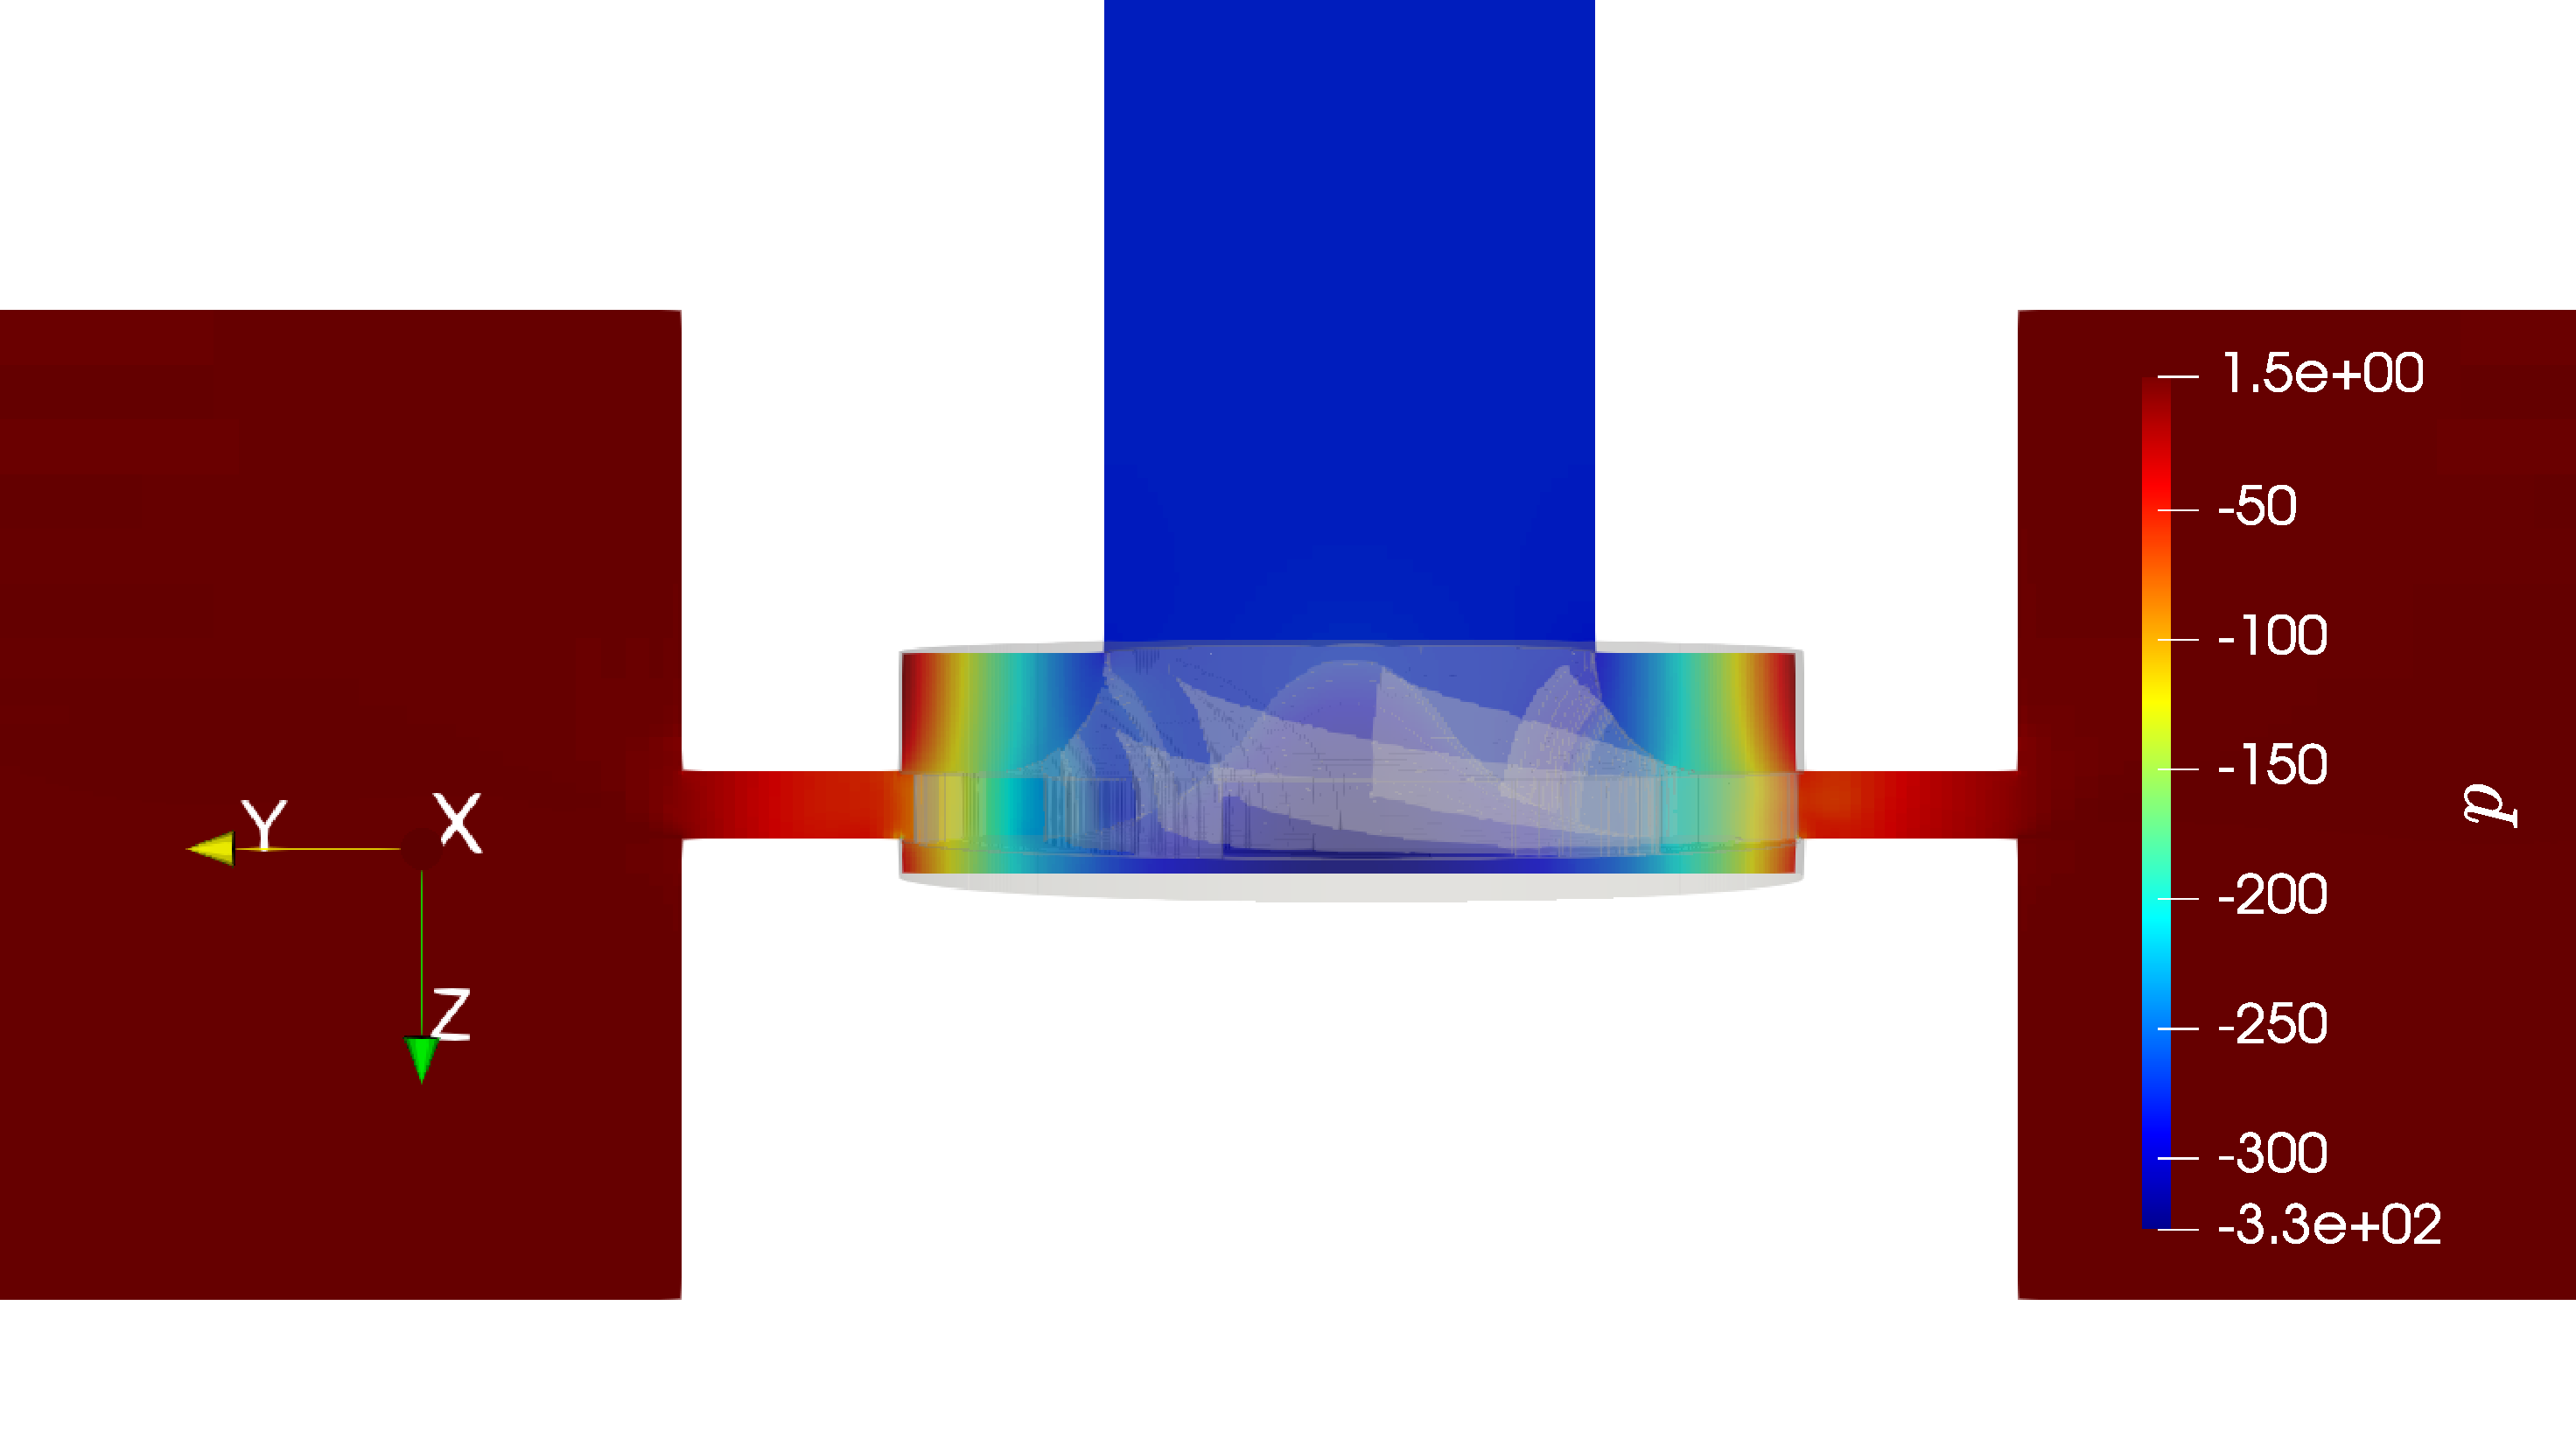
\includegraphics[width=0.9\textwidth]{figures/pressure_verProfile.pdf}
        \end{column}
    \end{columns}
    
\end{frame}
\section{Prospects}

\begin{frame}{Prospects}

    \begin{itemize}
        \item Perform Data Assimilation (DA) to \structure{\textbf{optimize the Immersed Boundary Method (IBM) penalty parameters}}, $\eta = (\boldsymbol{\eta_u}, \eta_\mathcal{K}, \eta_\omega)$, in order to better align the simulated flow profiles with the \structure{\textbf{PIV measurements}}
    \end{itemize}

    \begin{columns}
        \begin{column}{0.7\linewidth}
            \centering

            % \vspace{-0.1cm}

            % Adjust height (4cm here) as needed
            \footnotesize

            \begin{columns}
                \begin{column}{0.8\linewidth}
            Time- and azimuthally-averaged PIV measurements ($V_r$, $V_\theta$, and $V_z$) to enable meaningful comparison with the Multiple Reference Frame (MRF) simulation results
                \end{column}

                %\hspace{-1.8cm}
                
                \begin{column}{0.2\linewidth}

                \centering
                \footnotesize{code} \\ 
\includegraphics[scale=0.1]{logos/qrcode_github.com.png}
                \end{column}
            \end{columns}

            %\vspace{0.3cm}
            
            \only<1>{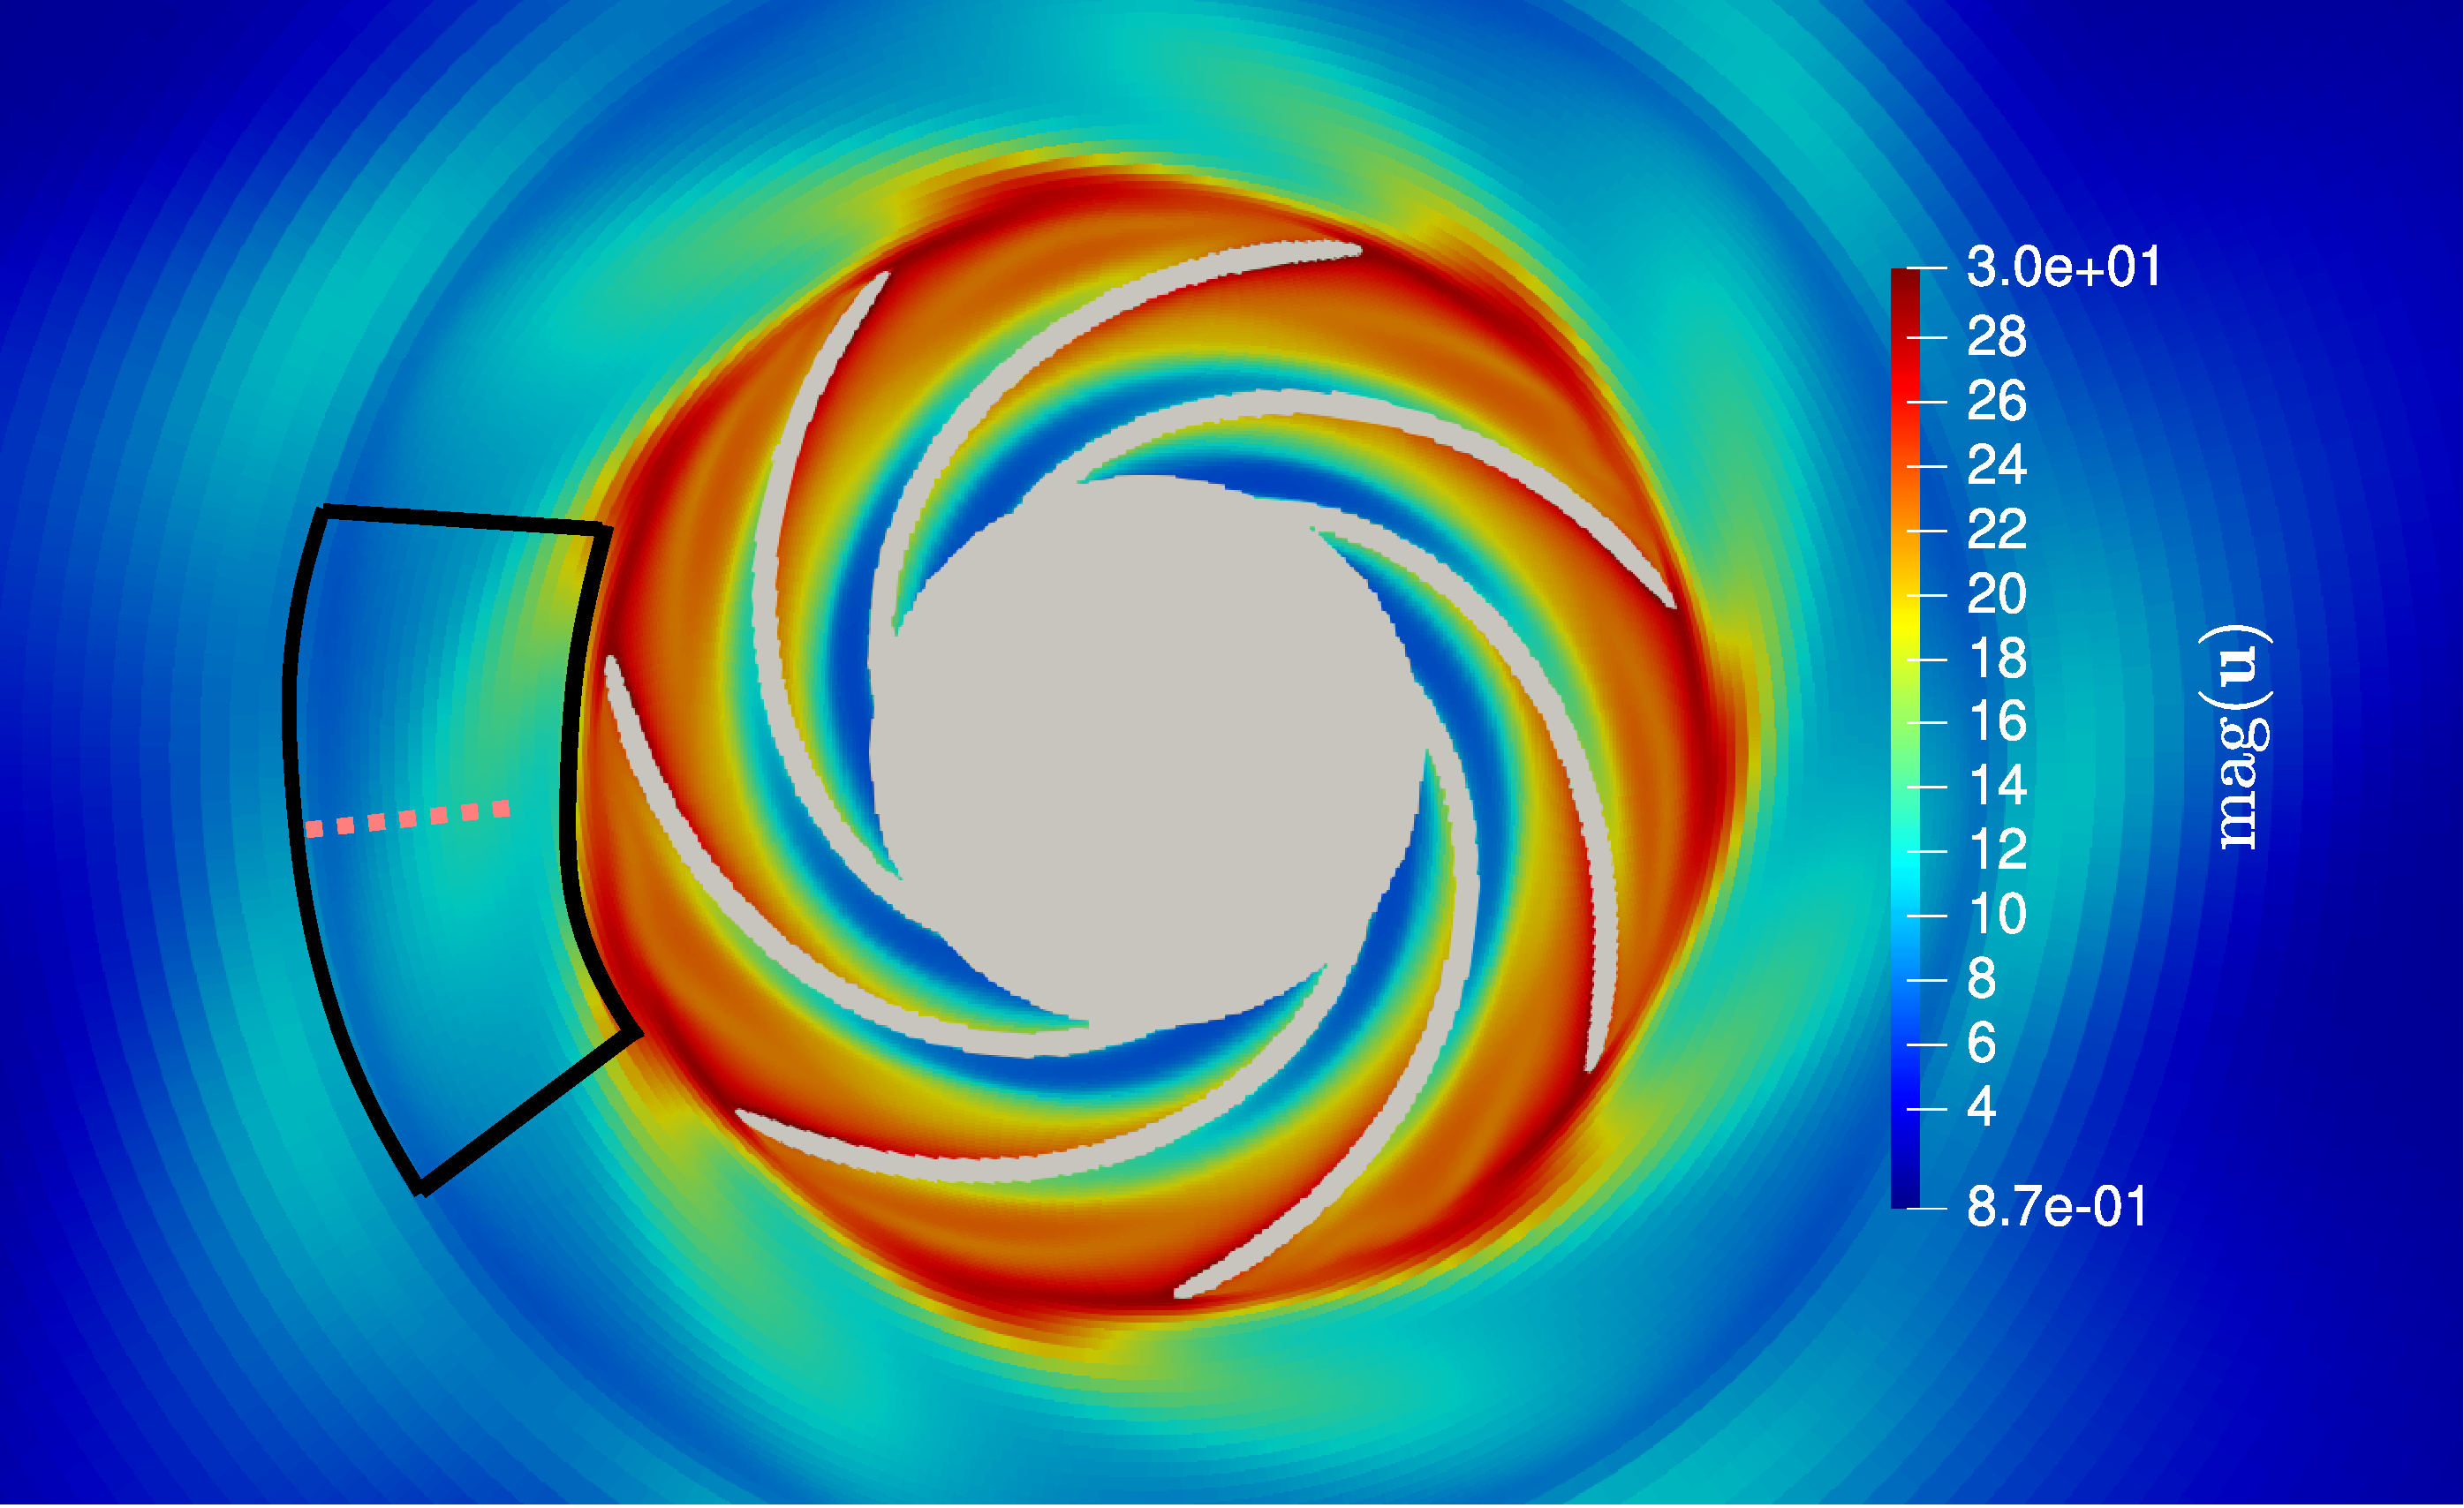
\includegraphics[scale=0.125]{figures/observations.pdf}}
            \only<2>{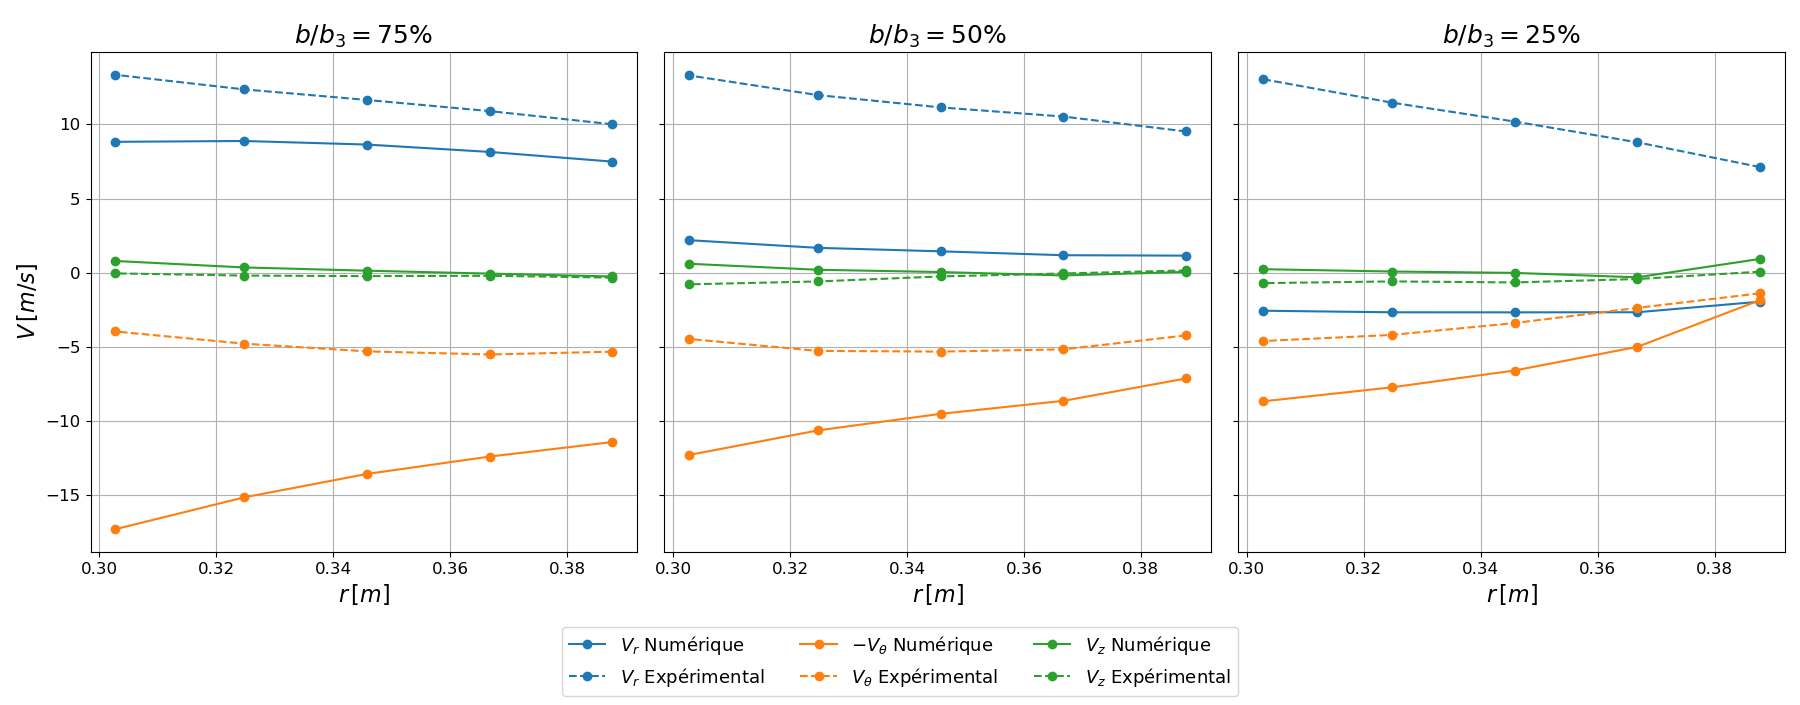
\includegraphics[scale=0.225]{figures/numVSxp.png}}
        \end{column}
        \begin{column}{0.3\linewidth}
            \centering
            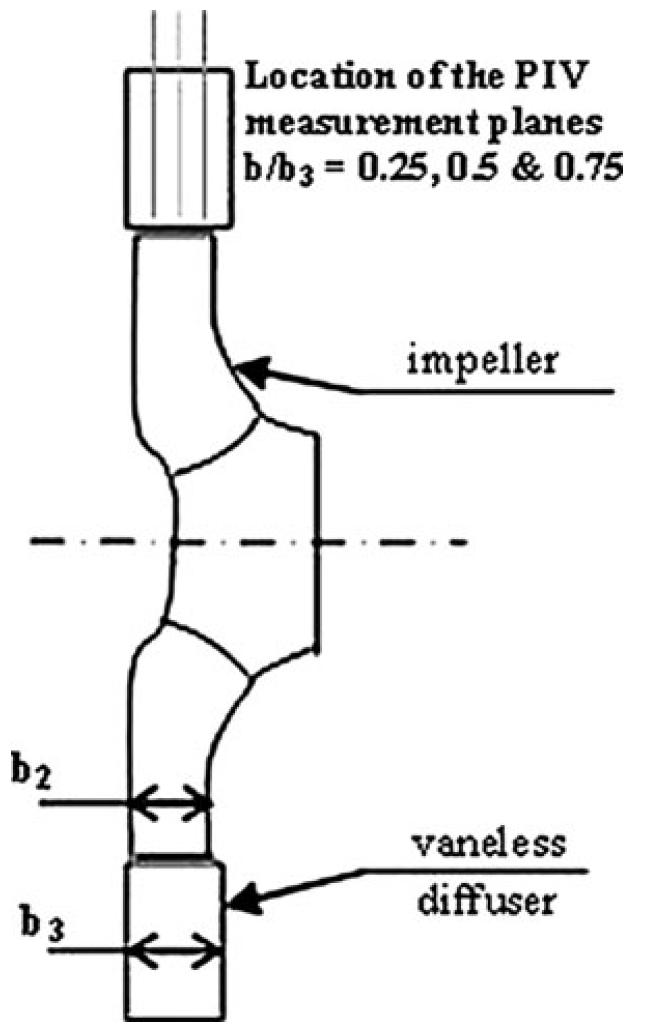
\includegraphics[scale=0.4]{figures/impeller_position.png}
        \end{column}
    \end{columns}
\end{frame}

\begin{frame}{Prospects}

    \begin{block}{\textbf{Future outlook}}
In the coming years, there is a strong potential to \structure{combine Data Assimilation (DA) and Machine Learning (ML) techniques} to develop a real-time \structure{\textbf{Digital Twin}} for active flow control in industrial applications
\end{block}

\begin{columns}
    \begin{column}{0.7\linewidth}
        \centering
        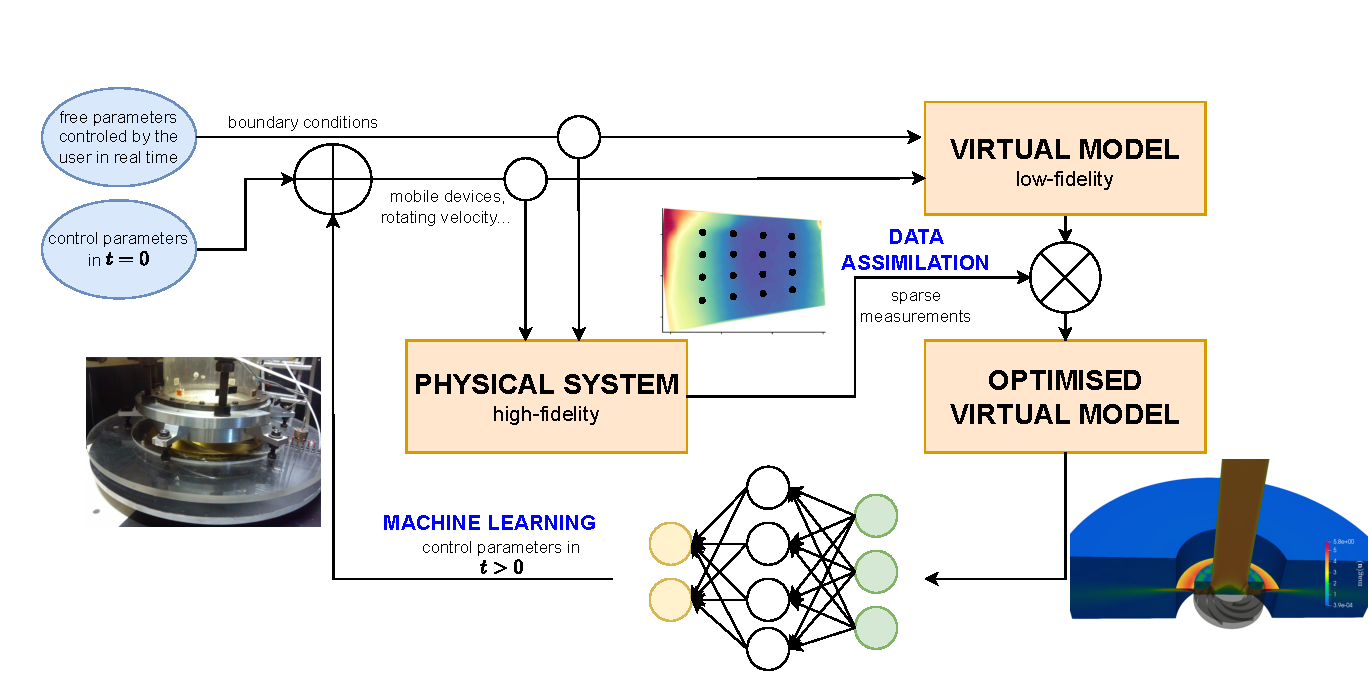
\includegraphics[scale=0.45]{figures/Digital_Twin_pump.pdf}
    \end{column}
    \begin{column}{0.3\linewidth}
        \begin{itemize}
            \item Increment efficiency and waste reduction
            \item Simplify predictive maintenance
            \item Optimize energy consumption
        \end{itemize}
    \end{column}
\end{columns}
    
\end{frame}

\begin{frame}

\begin{tikzpicture}[overlay,remember picture]
\node[right=0.2cm, yshift=-1cm] at (current page.150){
	
\includegraphics[width=3.5cm]{logos/Logo ENSAM.png}
};
\end{tikzpicture}

\begin{tikzpicture}[overlay, remember picture] 
  \node [xshift=0cm, yshift=-1cm] at (current page.90)
  {

\includegraphics[width=3.5cm]{logos/OpenFOAM_logo.png}
};		 
\end{tikzpicture}

% \begin{tikzpicture}[overlay, remember picture] 
%   \node [xshift=0.9cm, yshift=-1.2cm] at (current page.70)
%   {
% \includegraphics[width=2cm]{logos/ercoftac.jpg}
% };		 
% \end{tikzpicture}

\begin{tikzpicture}[overlay,remember picture]
\node[left=0.2cm, yshift=-1cm] at (current page.30){
	
\includegraphics[width=2.5cm]{logos/Logo LMFL.png}
};
\end{tikzpicture}

  \vspace{1cm}
  \centering \Huge
  \emph{Thanks for your attention!}

  \begin{center}
    \movie[externalviewer]{\normalsize{CLICK FOR VIDEO}}{pump.mov} \\
   \end{center}

\normalsize{
\textbf{Special acknowledgments: }
\begin{itemize}
    \item ANR (project ANR-JCJC-2021 IWP-IBM-DA)
    \item HPC resources of GENCI (project A0162A01741 on the IRENE supercomputer)
    \item LMFL experimental group, particularly Meng FAN, Antoine DAZIN, Gérard BOIS, and Francesco ROMANÒ
\end{itemize}}

\begin{figure}
    \begin{tabular}{cc}
    
\includegraphics[width=0.15\linewidth, trim = {0 8cm 0 3.6cm}, clip]{logos/ANR-logo-C.jpg} \qquad
    
\includegraphics[width=0.15\linewidth]{logos/tgcc-logo.png}
    \end{tabular}
\end{figure}
\end{frame}

\end{document}